\chapter{Алгоритмы проецирования визуальных данных на плоскость движения БТС}\label{ch:ch2}

В главе~\cref{ch:ch1} была показана необходимость комплексирования данных для построение более точной модели окружающего пространства. В данной главе предлагаются алгоритмы, реализующие комплексирование данных с RGB-камер и лидаров, установленных на БТС. Вначале предложен алгоритм оценки положения объектов, обнаруженных на изображении с камеры, в трёхмерном пространстве с использованием только данных с камеры и показана ограниченность качества его работы. Затем предложен алгоритм для решения той же задачи, но с использованием комплексирования данных с камеры и лидаров. Наконец предложен алгоритм проецирования информацию о свободной проезжей части с изображения на плоскость движения БТС.

\section{Алгоритм проекции визуальных детекций на плоскость движения БТС на основе модели L-Shape}\label{sec:ch2/sec1}

В данном разделе описан метод определения положения транспортных средств (наиболее распространенного типа объектов окружения в городских условиях) в виде произвольно ориентированных ограничивающих рамок на виде сверху (birds’-eye view) по изображению, полученному с одной монокулярной камеры. Этот метод состоит из двух этапов. На первом этапе вычисляется проекция видимой границы транспортного средства в виде сверху на основе двумерных детекций (2D-детекций) препятствий и сегментации проезжей части на изображении. Предполагается, что полученная проекция представляет зашумленные измерения двух ортогональных сторон ТС. На втором этапе строится ориентированная ограничивающая рамка вокруг полученной проекции. Для этого этапа будет предложен новый алгоритм построения рамки на основе предположения об L-образности проекции: L-Shape алгоритм.

\subsection{Этап 1. Проекция двумерной детекции изображения на вид сверху}\label{sec:ch2/sec1.1}

Пусть имеется изображение, зарегистрированное камерой БТС, с известной внутренней и внешней калибровкой. На этом изображении
производится двумерное детектирование ТС и семантическая сегментация проезжей части. Используя полученные данные, мы хотим достроить положение, ориентацию и габариты обнаруженных ТС на виде сверху. Далее описаны два подхода к определению границ окружающий ТС на плоскости движения БТС. 

\textbf{Наивный подход}

Пусть дан набор ограничивающих рамок на зарегистрированном изображении, полученный с помощью нейросетевой модели YOLOP~\cite{wu2022yolop}, осуществляющей детекцию ТС на изображении. Для дальнейшего определения положения обнаруженных ТС вводятся два предположения:

\begin{enumerate}
	\item  Все объекты находятся на земле (проезжей части дороги).
	\item  Поверхность дороги плоская. Далее в работе используется система координат, в которой уравнение плоскости, в которой лежит данная поверхность, имеет виде $z = 0$.
\end{enumerate}

Для оценки 3D-координат ТС, мы проецируем два нижних угла ограничивающей рамки на плоскость дороги(рис.~\cref{fig:proj3d}). Мы считаем известными параметры внутренней калибровки и внешней калибровок, поэтому данная операция происходит в два шага: сперва мы находим однородные координаты $p_u$ интересующих нас точек в системе локальной системе координат камеры, а затем, используя внешнюю калибровки, проецируем полученные точки на плоскость движения БТС: $z_l=0$ в системе $O_l$, получая окончательный результат $p_l$. Алгоритмы планирования пути зачастую работают с представлением объектов в виде геометрических фигур с ненулевой площадью или объёмом~\cite{petrovskaya2008model}. Для таких алгоритмов мы производим достраивание полученного отрезка до прямоугольника, добавлением к нему ортогональных отрезков фиксированной длины.

\begin{figure}[ht!]
	\centering
	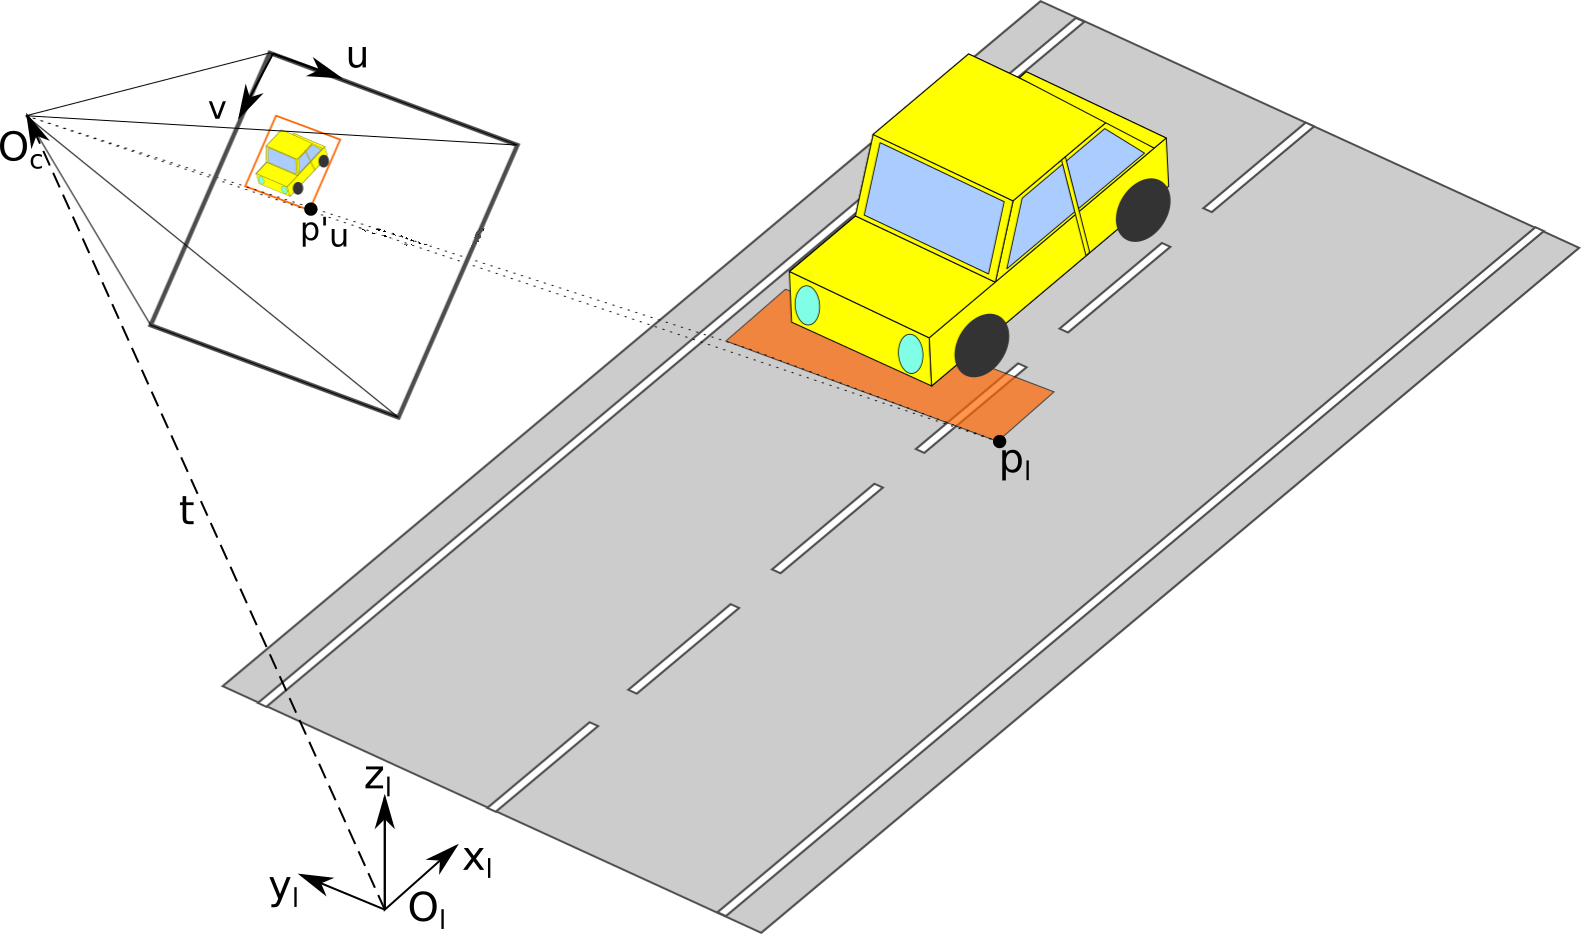
\includegraphics[width=0.8\textwidth]{images/l-shape-projection.png}
	\caption{Наивный подход к проецированию ограничивающей рамки в 2D на вид сверху.}
	\label{fig:proj3d}
\end{figure}


Данный алгоритм достаточно хорошо справляется с проецированием небольших объектов, например, людей, а также объектов, которые находятся в центре кадра и ориентированы вдоль оптической оси камеры. Однако, если объект большой и его границы не параллельны осям изображения, алгоритм проецирует его неверно, что может вызвать в алгоритмах планирования движения, использующих выходные данные из нашего алгоритма решение произвести остановку там, где она не требуется, т.к. возможен объезд. Пример такой ситуации показан на рис.~\cref{fig:blocked_trajectory}.

\begin{figure}[ht!]
	\centering
	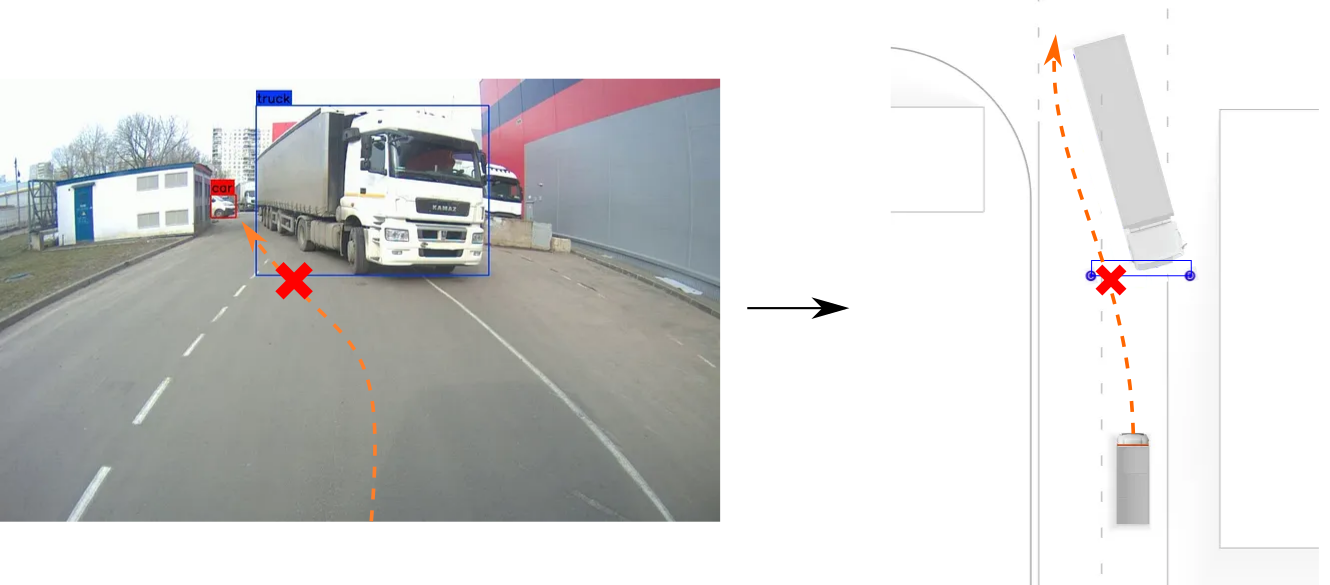
\includegraphics[width=0.8\textwidth]{images/blocked_trajectory.png}
	\caption{Неверная проекция грузовика. Зона слева от грузовика воспринимается, как часть объекта, и мешает объехать его.}
	\label{fig:blocked_trajectory}
\end{figure}

\textbf{Уточнение положения объекта с помощью семантической сегментации проезжей части}

Для решения продемонстрированной проблемы, мы дополнительно уточняем положение детектируемых объектов с учетом сегментации проезжей части (также полученной с помощью нейросетевой модели YOLOP). В результате наш алгоритм выглядит следующим образом:

\begin{enumerate}
	\item Берем $N$ равномерно распределенных точек на нижней границе ограничивающей рамки.
	\item Каждая полученная точка сдвигается к верху изображения пиксель за пикселем, пока она не выйдет за пределы проезжей части либо не достигнет верхнего края ограничивающей рамки.
	\item Выпуклая оболочка полученных точек проецируется на дорогу аналогично наивному подходу. 
\end{enumerate}

На рис.~\cref{fig:lshape} приведена демонстрация принципа работы алгоритма.

\begin{figure}[ht!]
	\centering
	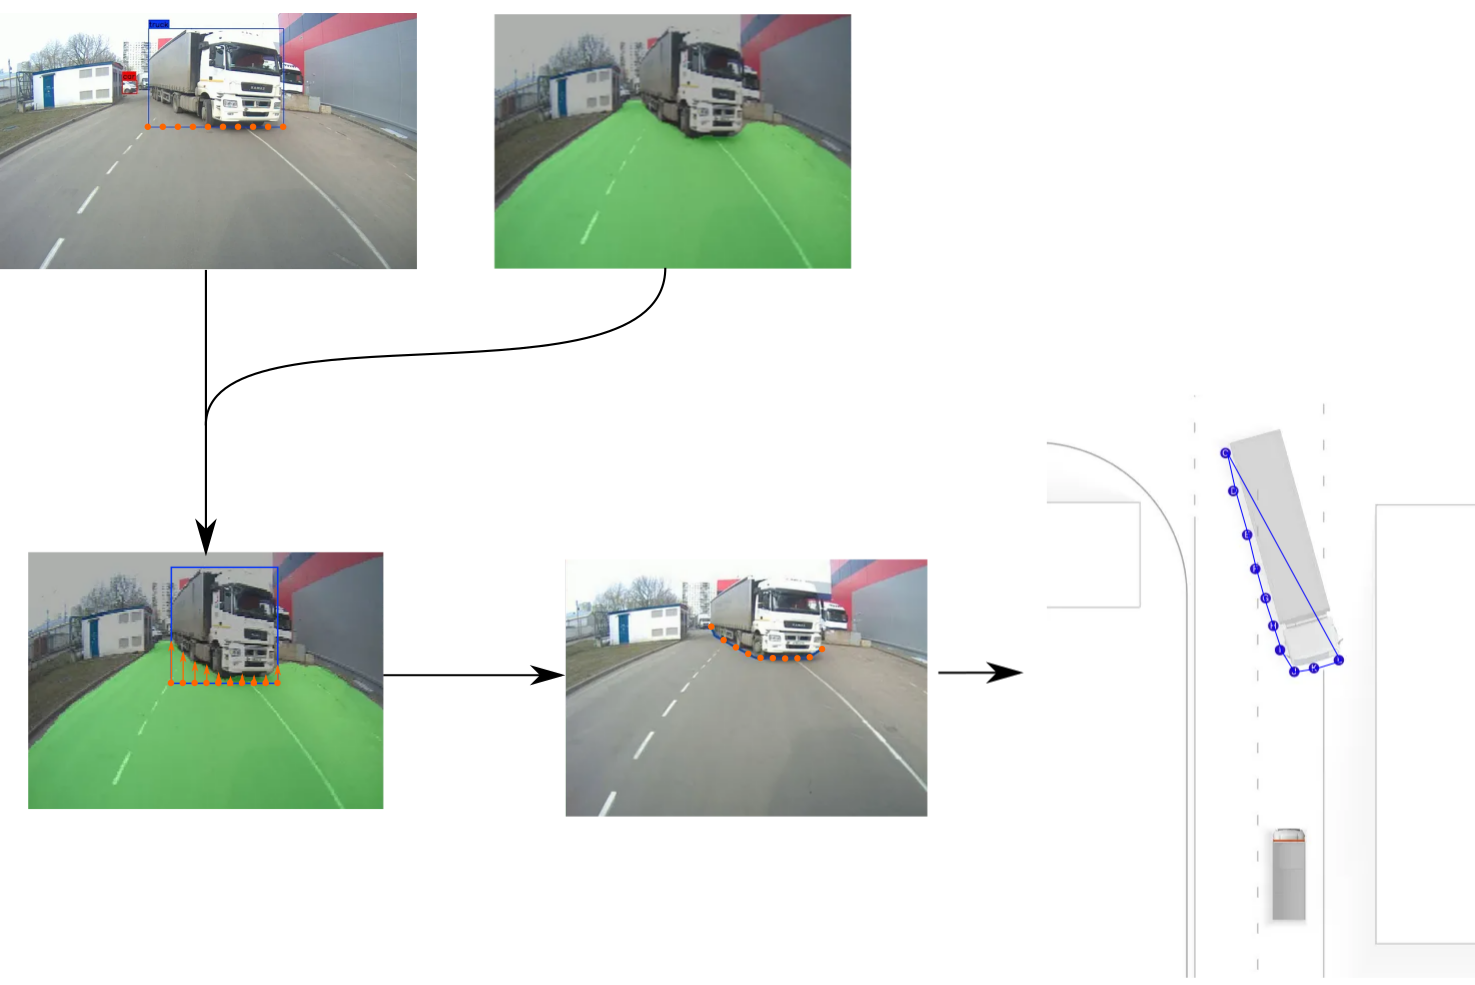
\includegraphics[width=\textwidth]{images/l-shape.png}
	\caption{Проекция двумерной ограничивающей рамки на вид сверху с учетом сегментации проезжей части.}
	\label{fig:lshape}
\end{figure}

Несмотря на недостатки этого метода, включая ошибки, вызванные изменяющимся зазором между ТС и дорогой, он может быть применим как способ построения одного из кандидатов для более сложных детекторов, учитывающих результаты работы нескольких алгоритмов, как это сделано в работе~\cite{Wang2021}

\subsection{Этап 2. Вписывание проекции объекта на виде сверху в ориентированную ограничивающую рамку.}

На следующем этапе алгоритма полученная на прошлом шаге проекция вписывается в ориентированную рамку на плоскости дороги. Такое представление упрощает работу последующим алгоритмам, работающим с полученными трехмерными детекциями, в частности некоторым алгоритмам планирования пути и многим алгоритмам отслеживания объектов Помимо этого, из-за окклюзии мы не можем видеть некоторые части детектируемого ТС из-за чего получаемая проекция покрывает только часть реально занимаемого им пространства. 

Для построения ограничивающей рамки мы делаем дополнительные предположения об L-образности вписываемых точек: 

\begin{enumerate}
	\item Вписываемые в рамку точки -- зашумлённые точки, принадлежащие двум смежным и ортогональным сторонам ТС
	\item Точки упорядочены таким образом, что сперва идут точки принадлежащие одной стороне ТС, затем точки второй стороны.
\end{enumerate}
Далее в работе данную модель мы будем именовать L-Shape моделью. Используя данную модель, нахождение ограничивающей рамки сводится к поиску двух перпендикулярных прямых: $l: y = kx + d_1$ и $l': x = -ky+d_2$, таких что минимизируется среднеквадратичная ошибка(mean squared error, MSE) вписываемых точек до соответствующей прямой. Согласно выбранной модели:

\begin{align*}
	\exists m \in \{1,\dots,N - 1\}\hookrightarrow& \forall i \in \{1,\dots,m\}, p_i = (x_i, y_i) \in l;\\
	&\forall i \in \{m+1,\dots,N\},p_i = (x_i, y_i) \in l'
\end{align*}

При этом заранее значение $m$ неизвестно. Задачу минимизации среднеквадратичной ошибки можно записать в следующем виде:

\begin{equation*}
	\operatorname*{argmin}_{k, d_1,d_2}\left(\begin{pmatrix}
		x_1 & 1 & 0 \\
		x_2 & 1 & 0 \\
		\vdots & \vdots  & \vdots  \\
		x_{m} & 1 & 0 \\
		-y_{m + 1} & 0 & 1 \\
		\vdots & \vdots  & \vdots  \\
		-y_{N} & 0 & 1 \\
	\end{pmatrix} 
	\begin{pmatrix}
		k \\
		d_1\\
		d_2 \\
	\end{pmatrix} - \begin{pmatrix}
		y_1 \\
		y_2\\
		\vdots \\
		y_{m} \\
		x_{m + 1} \\
		\vdots \\
		x_{N} \\
	\end{pmatrix}\right)^2    
\end{equation*}

Введя дополнительные обозначения, мы можем переписать это выражение следующим образом:

\begin{equation*}
	\operatorname*{argmin}_{a}\left(\begin{pmatrix}
		\widehat{x} & 1 & 0 \\
		-\widehat{y} & 0 & 1 \\
	\end{pmatrix} 
	a - \begin{pmatrix}
		\widetilde{y} \\
		\widetilde{x} \\
	\end{pmatrix}\right)^2
\end{equation*}

И далее:

\begin{equation*}
	\operatorname*{argmin}_{a}\left(Xa - y \right)^2
\end{equation*}

Решением данной задачи минимизации является:

\begin{align}
	a^* &= \left(X^TX\right)^{-1}X^Ty \label{eq:optimal_lsh_sol}\\
	\text{MSE} &= a^{*T}X^TXa - 2 a^{*T}X^Ty - y^Ty \label{eq:optimal_lsh_sol_mse}
\end{align}

Таким образом, неэффективная реализация модели L-Shape следующая: 

\begin{enumerate}
	\item Перебираем все значения $m \in \{1,\dots,N-1\}$
	\item Пересчитываем матрицы $X,y$
	\item Находим $a^*$, среднеквадратичная ошибка для каждой задачи минимизации по формулам~\cref{eq:optimal_lsh_sol},\cref{eq:optimal_lsh_sol_mse}
	\item В качестве финального решения для $l, l'$ выбираем $a^*$ с наименьшей среднеквадратичной ошибкой.
	\item Обрамляем вписываемый набор точек линиями параллельными $l$ и $l'$. Область ограниченная полученными линиями -- искомая ограничивающая рамка.
\end{enumerate}

Вычисление шагов 2 и 3 занимает $\Theta(N)$ операций. Эти шаги повторяются в цикле $N-1$ раз. Итоговая сложность такой реализации -- $\Theta(N^2)$. Покажем, как ускорить данный алгоритм. Для этого вычислим некоторые промежуточные матрицы, используемые при вычислении $a^*$ и среднеквадратичной ошибки (для удобства чтения введём обозначение $\overline{m} = N - m$):

\begin{align*}
	X^TX &= \begin{pmatrix}
		\sum{\widehat{x}^2} + \sum{\widehat{y}^2}& \sum\widehat{x} & -\sum\widehat{y} \\
		\sum\widehat{x} & m & 0  \\
		-\sum\widehat{y} & 0 & \overline{m}
	\end{pmatrix}\\
	\Delta_{X^TX} &= m \overline{m}(\sum{\widehat{x}^2} + \sum{\widehat{y}^2}) - m\left(\sum{\widehat{y}}\right)^2 - \overline{m} \left(\sum{\widehat{x}}\right)^2 \\
	\left(X^TX\right)^{-1} &=  \frac{1}{\Delta_{X^TX}} \\ &\begin{pmatrix}
		m \overline{m}& -\overline{m} \sum\widehat{x} & m \sum\widehat{y} \\
		-\overline{m} \sum\widehat{x} & \overline{m} (\sum{\widehat{x}^2} + \sum{\widehat{y}^2}) - \left(\sum\widehat{y}\right)^2& -\sum\widehat{x} \sum\widehat{y} \\
		m\sum\widehat{y} & -\sum\widehat{x} \sum\widehat{y} & m (\sum{\widehat{x}^2} + \sum{\widehat{y}^2}) - \left(\sum\widehat{x}\right)^2 \\
	\end{pmatrix}\\
	X^Ty  &= \begin{pmatrix}
		\widehat{x}^T\widetilde{y} - \widehat{y}^T\widetilde{x} \\
		\sum\widetilde{y} \\
		\sum\widetilde{x} \\
	\end{pmatrix}
\end{align*}

Можно заметить, что если вычислить значения $\sum{\widehat{x}^2} + \sum{\widehat{y}^2}$, $\sum{\widehat{x}\widetilde{y}}$, $\sum{\widetilde{x}\widehat{y}}$, $\sum{\widehat{x}}$, $\sum{\widehat{y}}$, $\sum{\widetilde{x}}$, $\sum{\widetilde{y}}$ один раз для $m=1$ (за $\Theta(N)$ операций), то для каждого последующего $m$ при <<перемещении>> точки $(x,y)$ между прямыми $l$ и $l'$, перечисленные значения пересчитываются следующим образом:

\begin{align*}
	\sum{\widehat{x}^2} + \sum{\widehat{y}^2} &+= x^2 - y^2 \\
	\sum{\widehat{x}} &+= x \\
    \sum{\widehat{y}} &-= y \\
	\sum{\widetilde{x}} &-= x\\
	\sum{\widetilde{y}} &+= y \\
	\widehat{x}^T\widetilde{y} &+= xy \\
	\widehat{y}^T\widetilde{x} &-= xy \\
\end{align*}

Таким образом, за фиксированное число шагов мы можем пересчитать выписанные ранее матрицы. Зная эти матрицы, вычисление~\cref{eq:optimal_lsh_sol},\cref{eq:optimal_lsh_sol_mse} так же занимает фиксированное, независящее от $N$, количество операций. Итоговая временная сложность алгоритма: $\Theta(N) + (N-1)\Theta(1) = \Theta(N)$.
Алгоритм, вычисляющий ориентированную ограничивающую рамку, описанным выше способом мы далее будем называть L-Shape алгоритм.

\section{Исследование точности алгоритма проекции визуальных детекций на основе модели L-Shape}\label{sec:ch2/sec2}

Для оценки качества второго этапа алгоритма мы сравнили его с подходом, минимизирующем площадь вычисляемой рамки, а также с алгоритмами построения рамок для кластеров точек из статьи~\cite{Wang2021}, адаптированными под проекции на вид сверху. 

\subsection{Набор данных}

Сравнение алгоритмов выполнялось на наборе данных, полученном с БТС. Данный набор включает в себя реальные сцены из $4$-х различных локаций: складов открытого типа и закрытых территорий, и содержит $12$ последовательностей кадров, снятых в разные сезоны и время суток. Суммарный размер набора составил $93$ кадра. Примеры сцен из набора приведены на рис.~\cref{fig:lshape_test_data}. Каждая сцена, помимо RGB-изображений с монокулярной камеры содержит облака точек, полученные с двух $32$-х лучевых лидаров, в которых были вручную аннотированы (обрамлены ограничивающими параллелепипедами) все автомобили и пешеходы. Проекции полученных таким образом ограничивающих параллелепипедов автомобилей на вид сверху были взяты в качестве эталонных положений объектов.

\begin{figure}[ht!]
	\centering
	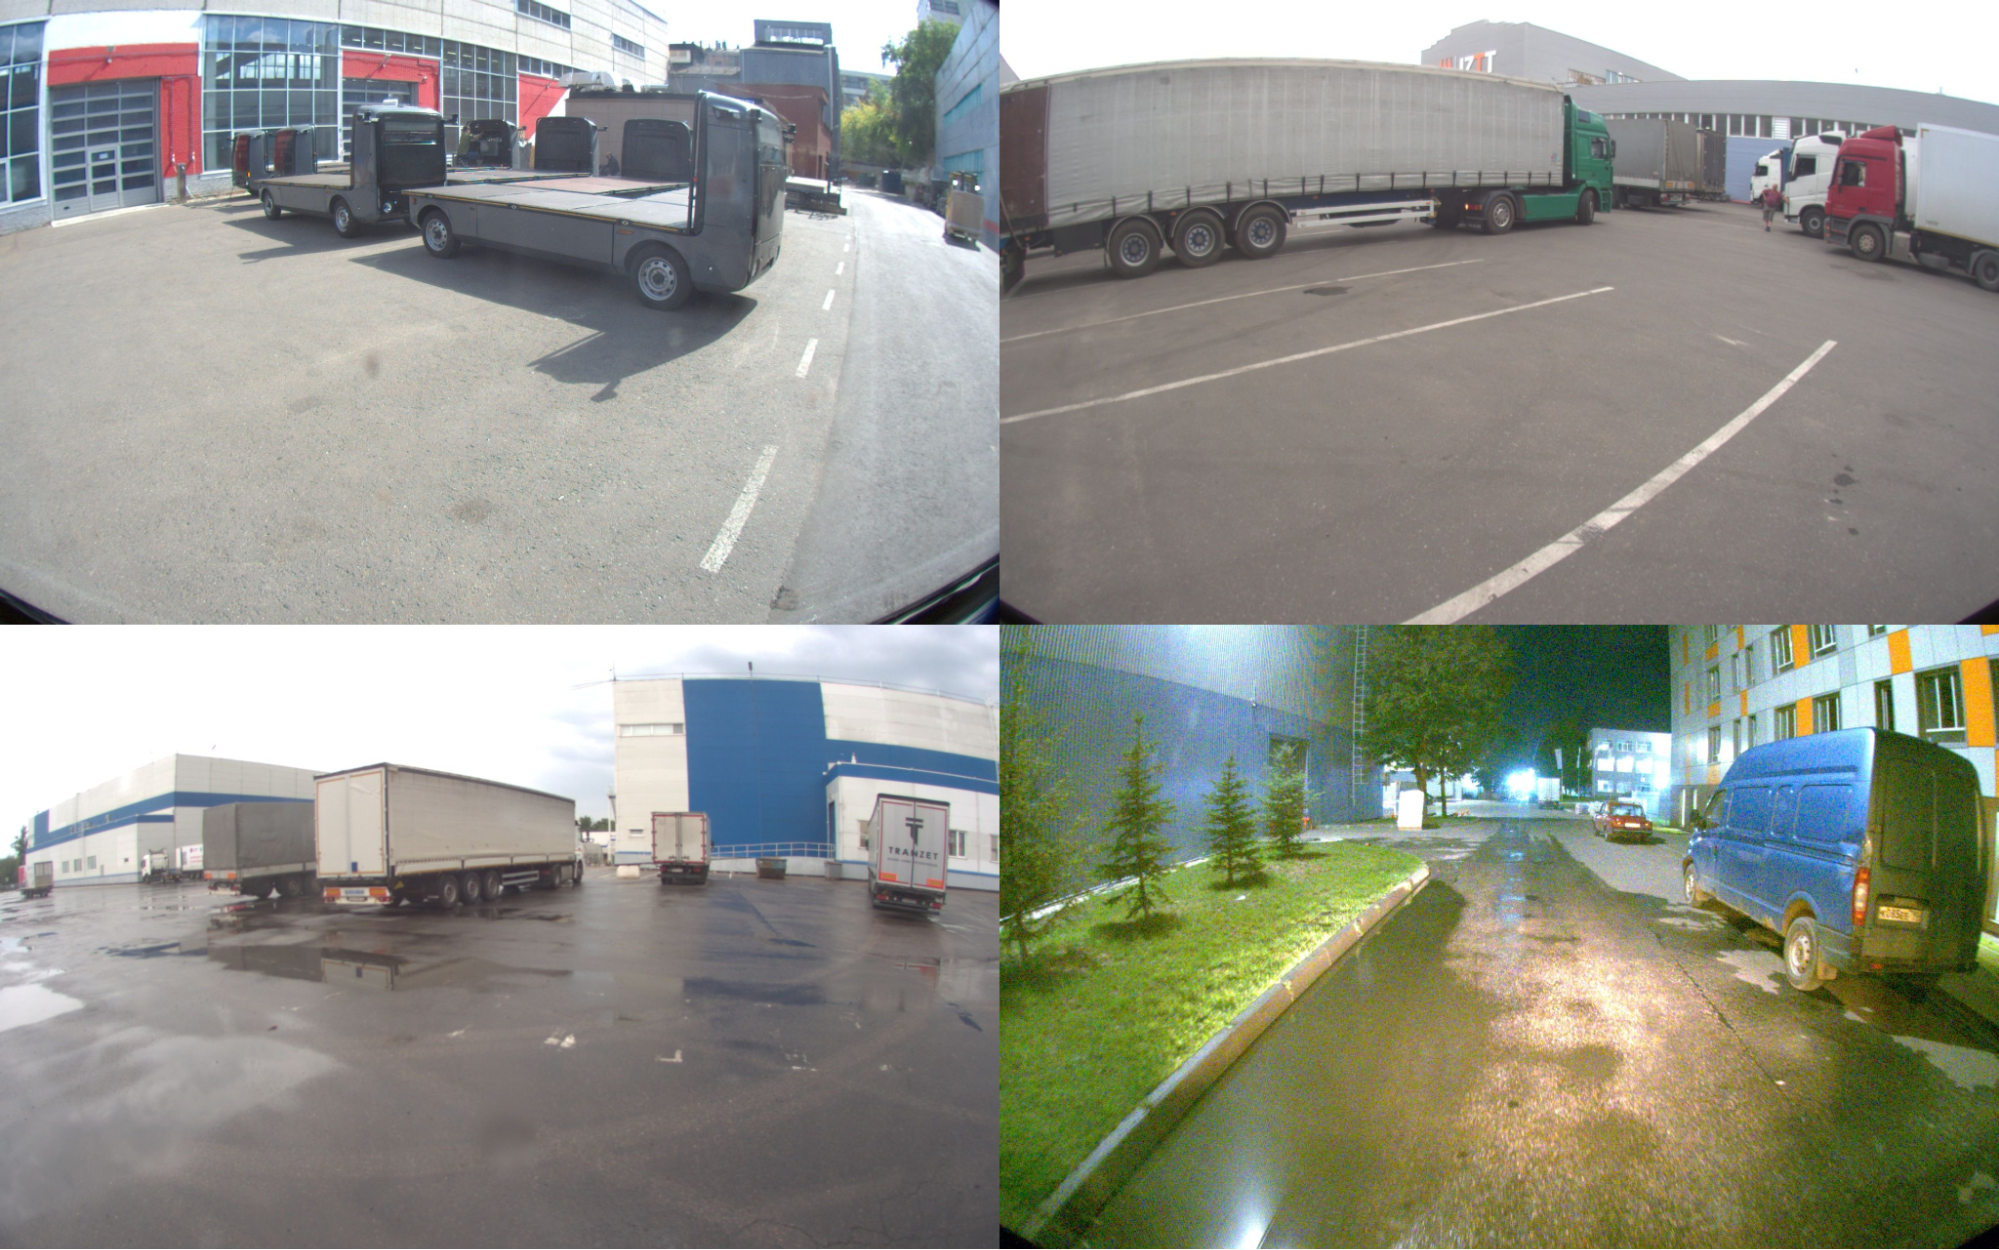
\includegraphics[width=\textwidth]{images/scenes.png}
	\caption{Проекция двумерной ограничивающей рамки на вид сверху с учетом сегментации проезжей части.}
	\label{fig:lshape_test_data}
\end{figure}

\subsection{Сравниваемые алгоритмы}

Для сравнения работы L-Shape алгоритма были взяты пять альтернативных подходов к решению задачи вписывания полигона в ориентированную ограничивающую рамку: подход, минимизирующий площадь итоговой рамки, и четыре подхода, описанные в работе~\cite{Wang2021}. Последние были разработаны для трехмерной детекции, в виде ориентированных ограничивающих параллелепипедов вокруг кластеров облаков точек. Отметим, что в статье~\cite{Wang2021} получаемые данными подходами детекции затем передавались в нейросетевую модель для создания итоговой трехмерной детекции. В рамках данной работы мы не рассматривали данную модель, ограничиваясь исследованием вычислительно эффективных алгоритмов, не требующих высоких вычислительных ресурсов (в частности, не требующих, наличия графических ускорителей). В работе Ванга~\cite{Wang2021} точки кластеров проецировались на вид сверху, затем для полученных проекций строилась выпуклая оболочка, и далее выполнялось её вписывание в ориентированную рамку на виде сверху (которая позже может быть достроена до параллелепипеда минимальной высоты, включающего все точки исходного кластера). Так как мы в качестве входа алгоритма использовали не кластеры точек, а проекции объектов на вид сверху, то мы адаптировали эти подходы под наши входные данные. 

\textbf{Построение рамки минимальной площади}

Тривиальным алгоритмом, решающим описанную задача является построение рамки, которая включает в себя все вписываемые точки и имеет наименьшую площадь. Пусть $(x_i,y_i), i \in \{1,\dots,N\}$ -- вершины выпуклой оболочки, указанные в порядке обхода. Алгоритм построения рамки минимальной площади опирается на то, что хотя бы одна сторона выпуклой оболочки принадлежит одной из сторон рамки. Для двумерного случая существует алгоритм с линейной временной сложностью по числу вершин $N$~\cite{arnon1983linear}.
Этот алгоритм правильно определяет положение транспортного средства (ТС) на дороге, только если среди точек оболочки есть хотя бы по одной точке каждой стороны ТС. На практике нам редко удается получить достаточное количество точек двух сторон, не говоря уже о трех сторонах. В таком случае, алгоритм выдаст неверное положение объекта, что может привести к нежелательным остановкам автономного ТС, использующего такой алгоритм, или, что еще хуже, автономная система может неправильно спланировать траекторию объезда препятствия. Пример такой ситуации представлен на рис.~\cref{fig:bad_estimation}. 
Несмотря на недостатки метода, он может быть применим как способ построения одного из кандидатов для более сложных детекторов, учитывающих результаты работы нескольких алгоритмов, как это сделано в работе~\cite{Wang2021}.

\begin{figure}[ht!]
	\centering
	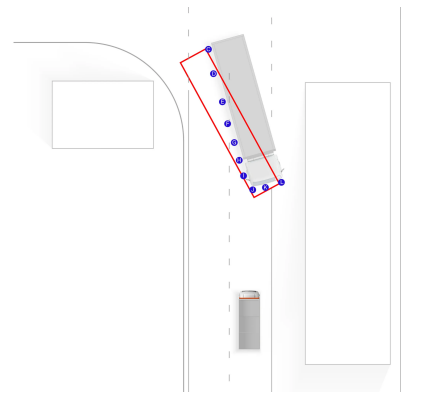
\includegraphics[width=0.7\textwidth]{images/bad_estimation.png}
	\caption{Пример неправильно построенной ограничивающей рамки.}
	\label{fig:bad_estimation}
\end{figure}

\textbf{Алгоритмы построения рамок для кластеров точек, адаптированные под проекции на вид сверху}

Из статьи Ванга~\cite{Wang2021} были взяты и адаптированы следующие алгоритмы вписывания полигона в ориентированную ограничивающую раму:

\begin{itemize}
	\item \textbf{Rotating Principal Component Analysis Algorithm.}
	Идея алгоритма заключается в том, чтобы взять собственные векторы, полученные в результате анализа главных компонент, и построить ограничивающую рамку минимального размера так, чтобы стороны этой рамки были параллельны полученным векторам.
	\item \textbf{Diagonal Principal Component Analysis Algorithm.}
	Этот алгоритм похож на предыдущий с той разницей, что собственный вектор, соответствующий наибольшему собственному значению, берется за основу диагонали рамки, а не ее сторон. Поэтому после того, как собственный вектор найден, алгоритм подбирает две точки оболочки, которые образуют прямую, наиболее близкую к направлению вектора. Затем алгоритм выбирает самую дальнюю от этой прямой точку и принимает эту точку за угол ограничивающей рамки. Ограничивающая рамка затем подгоняется и расширяется таким образом, чтобы заключить в себе все точки оболочки.
	\item \textbf{Longest Diameter Algorithm.} И снова этот алгоритм похож на предыдущий, но на этот раз диагональ ограничивающей рамки строится по самым дальним точкам оболочки, а собственный вектор не берется во внимание.
	\item \textbf{Rotated Triangle Algorithm.} В этом алгоритме перебираются пары соседних вершин выпуклой оболочки. Для каждой пары находится третья точка, максимально удалённая от прямой, проходящей через эту пару. Полученные три точки образуют треугольник. Среди всех построенных таким образом треугольников выбирается наибольшей площади, и соответствующая ему пара соседних вершин оболочки принимается за принадлежащую одной из сторон искомой рамки. Исходя из этого, можно достроить и расширить рамку, как это делалось при работе с другими алгоритмами.
\end{itemize}

\subsection{Описание эксперимента}

На изображениях из нашего набора данных запускался первый этап алгоритма, вычисляющий проекцию препятствия на вид сверху. Для сопоставления полученных проекций с эталонными данными вычислялись коэффициент Жаккара~\cite{app112411630} для каждой пары проекция-эталон, после чего применялся Венгерский алгоритм~\cite{kuhn1955hungarian}. 

Для каждой полученной проекции затем запускались все сравниваемые алгоритмы для второго шага алгоритма(L-Shape, рамка минимальной площади и алгоритмы из работы Ванга~\cite{Wang2021}), и для результирующего положения препятствия измерялся коэффициент Жаккара. Примеры полученных проекций, полученных ограничивающих рамок и эталонных положений представлены на рис.~\cref{fig:lshape-exp-demo}. 

\begin{figure}[ht!]
	\centering
	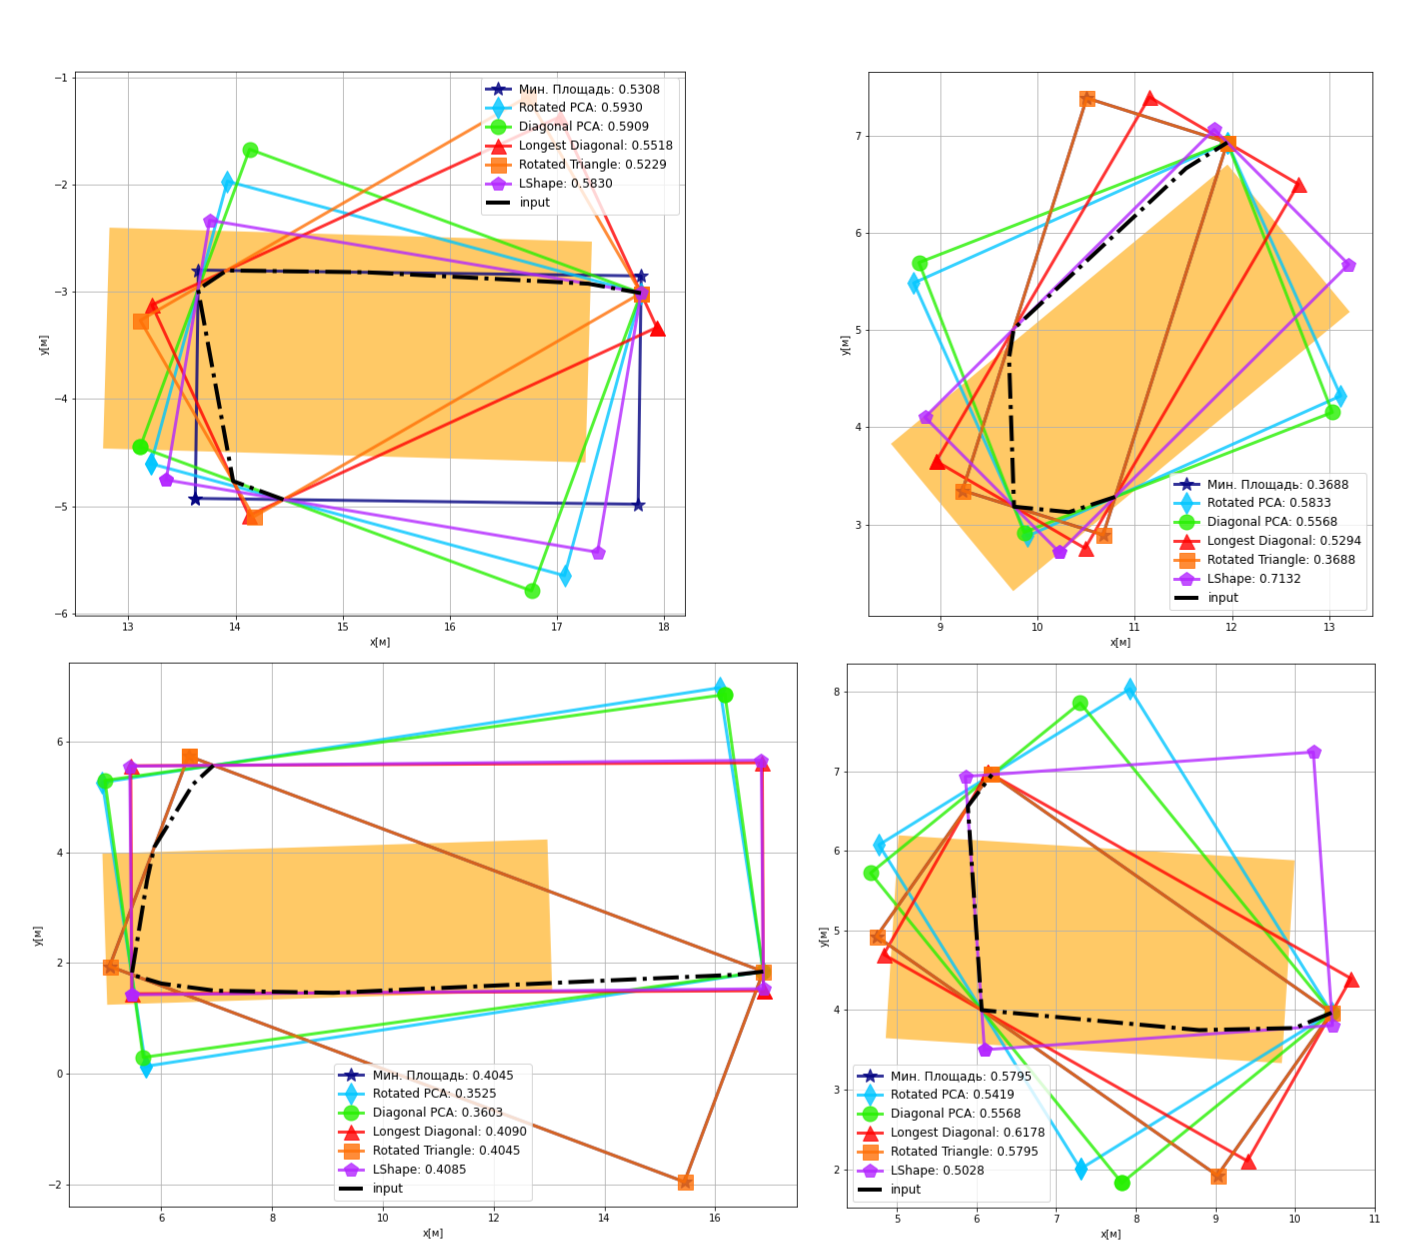
\includegraphics[width=0.8\textwidth]{images/l-shape-exp-demos.png}
	\caption{Примеры работы сравниваемых алгоритмов построения ограничивающих рамок.}
	\label{fig:lshape-exp-demo}
\end{figure}

\subsection{Результаты экспериментов.}

В таблице~\cref{tab:lshape-exp-res} представлена статистика измеренных коэффициентов Жаккара для каждого алгоритма. Можно видеть, что представленный алгоритм L-Shape превосходит по качеству другие исследуемые алгоритмы. Худшие результаты показал алгоритм Rotated Triangle. Однако само значение среднего коэффициента Жаккара сравнительно невелико в том числе и для представленного алгоритма L-Shape. Объясняется это в первую очередь ограниченной применимостью предположения о плоскости поверхности дороги, а также не идеальностью внешней калибровки камеры, вызванной наклоном дороги, загруженностью транспортного средства, изменившимся объемом шин и т.п. В результате предполагаемая плоскость дороги отклоняется от плоскости идеальной аппроксимации дороги и для удаляющихся препятствий наблюдается накопление ошибки. Помимо этого, погрешность первой части алгоритма: вычисления проекции объекта на вид сверху, выше для более удалённых объектов из-за линейной перспективы изображения. Чтобы учесть это, было предложено ограничить рабочее расстояние алгоритмов: не учитывать препятствия далее некоторого фиксированного порога. На Рис.~\cref{fig:lshape-metrics} представлен график зависимости среднего коэффициента Жаккара в зависимости от данного порога. Видно, что качество предсказываемого положения препятствия начинает падать после $10$~метров для всех рассматриваемых алгоритмов. Также можно видеть, что при всех значениях L-Shape алгоритм сохраняет первенство по измеряемой метрике.

\begin{table}[h!]
	\small
	\centering
	\begin{tabular}{|p{0.2\textwidth}|p{0.1\textwidth}|p{0.1\textwidth}|p{0.1\textwidth}|p{0.1\textwidth}|p{0.12\textwidth}|p{0.1\textwidth}|}
		\hline
		\textbf{Характеристика}          & \textbf{Мин. площадь} & \textbf{Rotating PCA} & \textbf{Diagonal PCA} & \textbf{Longest Diagonal} & \textbf{Rotated Triangle} & \textbf{L-Shape}\\
		\hline
		Среднее & $0,294\newline(-12,8~\%)$ & $0,328\newline(-2,7~\%)$ & $0,321\newline(-4,7~\%)$ & $0,323\newline(-4,2~\%)$ & $0,301\newline(-10,7~\%)$ & \boldmath$0,337\newline(-0,0~\%)$ \\
		\hline
		\tiny Среднеквадратичное\newline отклонение & $0,146$ & $0,144$ & $0,149$ & $0,156$ & $0,141$ & $0,141$ \\
		\hline
		Минимум & $0,059\newline(-24,4~\%)$  & $0,075\newline(-3,8~\%)$ & \boldmath$0,078\newline(-0,0~\%)$ & $0,074\newline(-5,1~\%)$ & $0,059\newline(-24,4~\%)$ & \boldmath$0,078\newline(-0,0~\%)$\\
		\hline
		$25$~\% & $0,198\newline(-13,9~\%)$ & $0,219\newline(-4,8~\%)$ & $0,202\newline(-12,2~\%)$ &$0,199\newline(-13,5~\%)$ & $0,208\newline(-9,6~\%)$ & \boldmath$0,230\newline(-0,0~\%)$ \\
		\hline
		$50$~\% & $0,257\newline(-21,6~\%)$ & $0,316\newline(-3,7~\%)$ & $0,316\newline(-3,7~\%)$ & $0,287\newline(-12,5~\%)$ & $0,264\newline(-19,5~\%)$ & \boldmath$0,328\newline(-0,0~\%)$ \\
		\hline
		$75$~\% & $0,383\newline(-15,1~\%)$ & $0,448\newline(-0,7~\%)$ & $0,445\newline(-1,3~\%)$ & $0,442\newline(-2,0~\%)$ & $0,425\newline(-5,8~\%)$ & \boldmath$0,451\newline(-0,0~\%)$ \\	
        \hline
        Максимум & $0,649\newline(-9,0~\%)$ & $0,607\newline(-14,9~\%)$ & $0,622\newline(-12,8~\%)$ & $0,651\newline(-8,7~\%)$ & $0,579\newline(-18,8~\%)$ & \boldmath$0,713\newline(-0,0~\%)$ \\
        \hline
	\end{tabular}
	\caption{Статистики полученных коэффициента Жаккара для сравниваемых алгоритмов.}
	\label{tab:lshape-exp-res}
\end{table}

\begin{figure}[ht!]
	\centering
	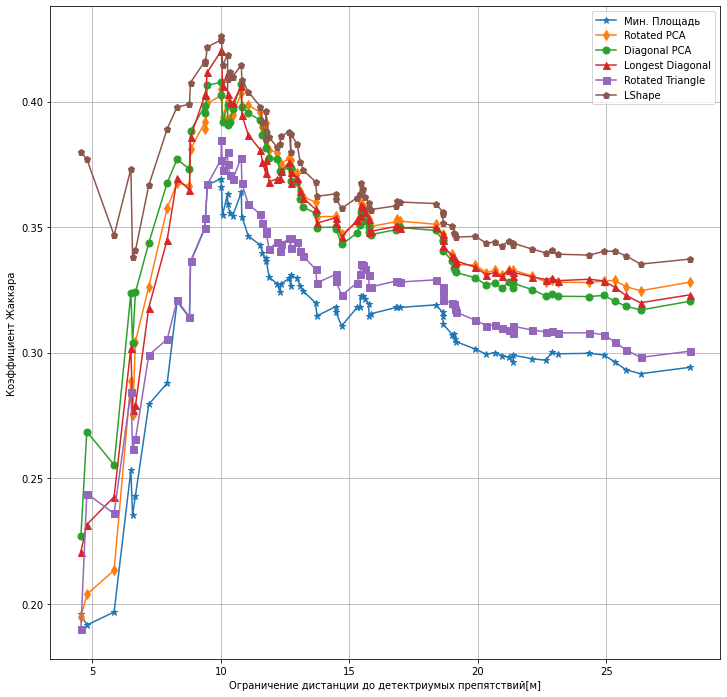
\includegraphics[width=\textwidth]{images/l-shape_metrics.png}
	\caption{График зависимости среднего коэффициента Жаккара от ограничения дистанции до детектируемых препятствий.}
	\label{fig:lshape-metrics}
\end{figure}


\section{Алгоритм проекции визуальных детекций на плоскость движения БТС на основе комплексирования визуальных и лидарных данных}\label{sec:ch2/sec3}

Одним из фундаментальных ограничений описанного в прошлом разделе L-Shape алгоритма является предположение о том, что поверхность проезжей части лежит в плоскости. В реальном мире это предположение не выполняется как в силу рельефа местности, в которой проложена дорога, так и согласно государственным стандартам и сводам правил, регулирующим конструктивные особенности дорожного покрытия. Так согласно СП 34.13330.2012\cite{sp34_2012} дорожное покрытие имеет двускатный поперечный профиль на прямых участках дороги и односкатный на виражах (см. рис.~\cref{fig:road_profile}).

\begin{figure}[ht!]
	\centering
	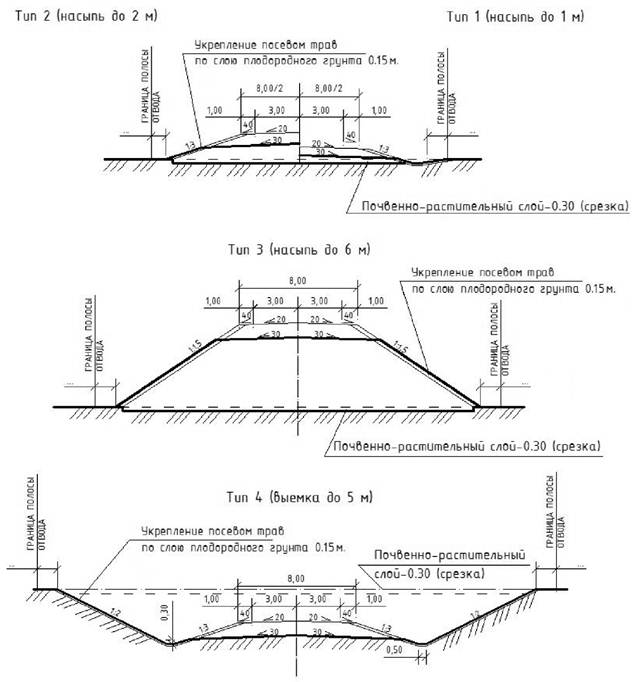
\includegraphics[width=0.7\textwidth]{images/road_profile.jpg}
	\caption{Примеры оформления поперечного профиля из ГОСТ 21.701-2013~\cite{gost217012013}.}
	\label{fig:road_profile}
\end{figure}

Для преодоления данного ограничения необходимо добавить источник информации, позволяющий оценить расстояние до наблюдаемых объектов без использования упомянутого предположения. В качестве такого источника информации были использованы механические лидары (лазерные дальномеры), установленные на БТС. Был разработан алгоритм комплексирования данных, полученных с камеры и лидаров, для оценки положения окружающих БТС объектов. Облако точек лидара представляет собой набор точек в трёхмерной системе координат лидара: $P_s = \{(x_i, y_i, z_i), i \in \{1,\dots, N_s\}\}$, где $s$ -- идентификатор лидара, $N_s$ -- количество зарегистрированных им точек. Все облака точек, а также изображения, полученные камерой, имеют временную метку момента регистрации датчиком. Сенсоры работают с фиксированной частотой и синхронизированы друг с другом. Это позволяет однозначно сопоставить данные  из последовательности измерений с датчиков в единые <<кадры>>, описывающие окружающую БТС сцену в конкретный момент времени. Далее будем считать, что все облака точек с каждого лидара:
\begin{enumerate}
	\item Приведены в локальную систему координат БТС $O_l$.
	\item Точки попадающие на БТС удалены, что возможно при известной геометрии БТС.
	\item Положение точек скорректировано и приведено к одному моменту времени, чтобы компенсировать собственное движение БТС во время регистрации облака точек.
	\item После предыдущих манипуляций облака объединены в одно общее облако точек $P$.
\end{enumerate}
После этих преобразований, один <<кадр>> представляет собой пару изображение--облако точек. В Листинге~\ref{alg:true3ddet} представлен алгоритм осуществляющий комплексирование данных одного кадра для оценки положения препятствий в окружающей БТС сцене: из облака выделяется подмножество точек, не принадлежащих  земле, производится объединение близко расположенных точек в кластеры, которые затем сопоставляются с двумерными детекциями, найденными на изображении. Наконец, кластеры, которым нашлось сопоставление среди детекций дополнительно фильтруется от точек, проецируемых за пределы соответствующей детекции и находится ограничивающий параллелепипед описанный вокруг полученного набора точек.  На рисунке~\cref{fig:true3ddet_demo} показан результат работы представленного алгоритма на данных, полученных с датчиков БТС. Отметим, что шаг 3 алгоритма~\ref{alg:true3ddet} был реализован в виде алгоритма с использованием параллельных вычислений на платформе CUDA (англ. Compute Unified Device Architecture)~\cite{cuda}. Данная реализация была предложена в работе Нгуена~\cite{nguyen2020fast}.

\begin{algorithm}
	\caption{Алгоритм определения положения объектов на основе комплексирования данных с камеры и лидаров.}
	\label{alg:true3ddet}
	\LinesNumbered
	\KwIn{$I$ -- изображение с RGB-камеры, $P$ -- облако точек.}
	\KwOut{$b_i$ -- ориентированные ограничивающие рамки на виде сверху окружающих БТС объектов.}
	Произвести поиск двумерных детекций объектов на $I$: $\{d_1,\dots d_n\}$\;
	Выделить в облаке точек $P$ точки, не принадлежащие поверхности земли: $P_o$\;
	Кластеризовать полученное облако точек $P_o$  с расстоянием Евклида: $P_o = \bigcup\limits_{i=1}^l C_i; C_i \cap C_j = \emptyset, i\neq j$\;
	Спроецировать все кластеры на изображение $I$: $C_i \rightarrow \widehat{C}_i$. Все точки проецируемые за границы $I$, а также находящиеся позади оптического центра камеры отбрасываются. Пустые после проекции кластеры -- удаляются\;
	Для каждого спроецированного кластера найти ограничивающую рамку минимального размера: $d_{C_i}$\;
	Используя Венгерский алгоритм найти наилучшее сопоставление найденных детекций $d_i$ с построенными ограничивающими рамками $d_{C_i}$, максимизирующий суммарный коэффициента Жаккара. Не сопоставленные кластеры -- удаляются.\;
	В оставшихся кластерах удалить точки, не попадающие при проекции в сопоставленную детекцию $d_i$: $C_i \rightarrow C^-_i$.\;
	\ForEach{$C^-_i$}{
		Используя RANSAC(RANdom SAmple Consensus)~\cite{fischler1981} найти прямую $l_i$, хорошо описывающую большую часть точек <<очищенного>> кластера $C^-_i$.\;
		Аналогично L-Shape алгоритму построить ограничивающую рамку $b_i$, со сторонами параллельными $l_i$ и ортогональной ей $l'_i$.\;
	}
	\Return{$\{b_i\}$}
\end{algorithm}

\begin{figure}[ht]
	\centering
	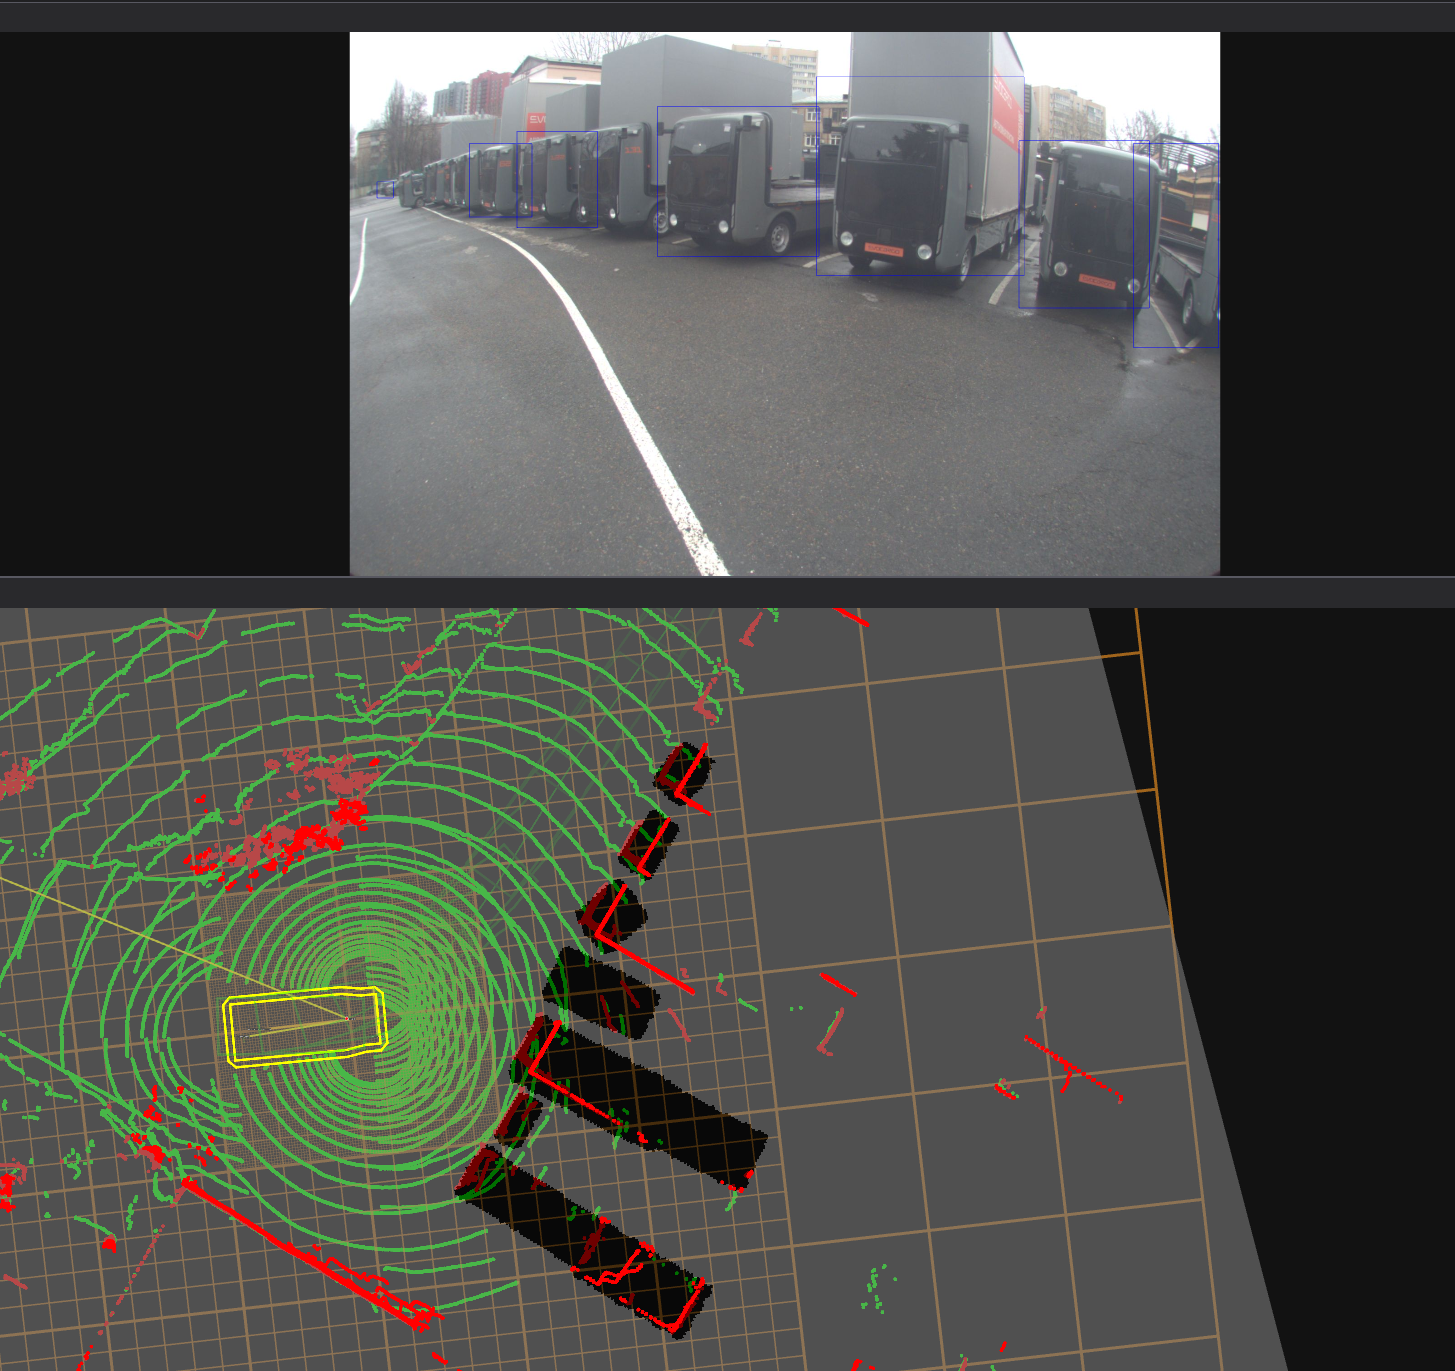
\includegraphics[width=0.8\textwidth]{images/true3ddet_demo}
	\legend{На верхнем изображении c камеры БТС прямоугольниками выделены двумерные детекции, полученные моделью YOLOP. На нижнем красными точками отмечены точки, зарегистрированные лидаром и классифицированные как точки препятствия. Полученные алгоритмом детекции показаны в виде чёрных прямоугольников.}
	\caption{Демонстрация работы алгоритма~\ref{alg:true3ddet} на данных, полученных с БТС.}
	\label{fig:true3ddet_demo}
\end{figure}

\subsection{Разделение облака точек на точки земли и препятствий}\label{sec:ch2/sec3.1}

Отметим нетривиальность шага 2 алгоритма~\ref{alg:true3ddet}. Зачастую такое разделение производится поиском с помощью RANSAC плоскости, хорошо описывающей часть точек в облаке. Однако, такой подход возвращает нас к предположению о совпадении поверхности дороги с некоторой плоскостью, от которого мы нацелены уйти. Поэтому в рамках данного алгоритма используется подход без использования поиска плоскостей.  В рамках данного подхода мы сперва производим поиск точек, для которых мы уверены, что они принадлежат земле. Далее мы решаем задачу регрессии: мы хотим найти зависимость высоты земли $z_l$ от координаты в плоскости движения БТС $(x_l, y_l)$. В качестве обучающей выборки используются выбранные нами в начале точки. В качестве тестовых точек берутся координаты $(x_l, y_l)$ входного облака точек. Мы решаем данную задачу регрессии на основе гауссовских процессов (Gaussian Process Regression, GPR)~\cite{rasmussen2003gaussian}.

Регрессия на основе гауссовских процессов представляет собой байесовский непараметрический подход к аппроксимации функции, задающей зависимость значения целевой переменной от вектора признаков. В рассматриваемой задаче целью является аппроксимация функции \( f: (x_l, y_l) \rightarrow z_l \), где \((x_l, y_l)\) -- координаты точки в плоскости движения БТС, а \( z_l \) -- соответствующая высота земли.

Гауссовский процесс задаётся как распределение на множестве функций и полностью определяется средним значением \( m(\mathbf{x}) \) и ковариационной функцией (ядром) \( k(\mathbf{x}, \mathbf{x}') \), где \( \mathbf{x} = (x_l, y_l) \). В нашем сценарии мы использовали ядро Матерна $(\nu=3/2)$~\cite{stein1999interpolation}, которое лучше справляется с аппроксимацией в точках разрыва функции(рисунок~\cref{fig:matern_justification}). Такие разрывы часто присутствуют в реальных сценах вокруг БТС, например, в местах соединения проезжей части и тротуаров.

$$k(\mathbf{x}, \mathbf{x}') = \sigma_f^2 \left(1 + \frac{\sqrt{3} d}{l}\right) \exp\left(-\frac{\sqrt{3} d}{l}\right),$$

где \( d = \|\mathbf{x} - \mathbf{x}'\| \) --- евклидово расстояние между точками, \( \sigma_f^2 \) --- вариация функции, а \( l \) --- гиперпараметр длины масштаба.

\begin{figure}[ht]
	\centering
	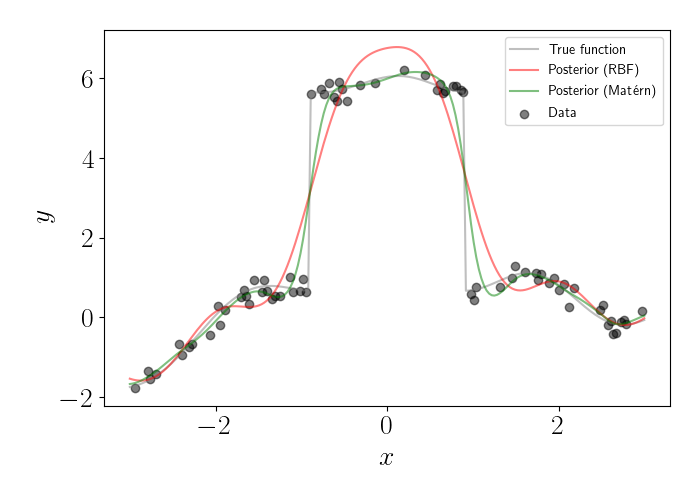
\includegraphics[width=0.7\textwidth]{images/matern_justification}
	\caption{Сравнение регрессии на основе гауссовских процессов с использованием в качестве ядра радиальной базисной функции и ядра Матерна~\cite{Andy_Jones_2021}.}
	\label{fig:matern_justification}
\end{figure}

Для обучающей выборки размером \( N_t \) с входами \( \mathbf{X} = \{\mathbf{x}_i\}_{i=1}^{N_t} \) и соответствующими наблюдениями высоты \( \mathbf{z} = \{z_i\}_{i=1}^{N_t} \) задача регрессии сводится к вычислению апостериорного распределения значений \( z_* \) для тестовых точек \( \mathbf{X}_* = \{\mathbf{x}_*\} \).

Обозначим ковариационные матрицы:

\begin{equation}
K = [k(\mathbf{x}_i, \mathbf{x}_j)]_{i,j=1}^{N_t}, \quad K_* = [k(\mathbf{x}_*,\mathbf{x}_i)]_{i=1}^{N_t}, \quad K_{**} = [k(\mathbf{x}_{*_i},\mathbf{x}_{*_j})]_{i,j=1}^{N},\label{eq:cov_gpr}
\end{equation}

тогда условное распределение предсказаний \( p(z_* \mid \mathbf{X}, \mathbf{z}, \mathbf{x}_*) \) является гауссовским с параметрами:

\begin{equation}
	\widehat{z} = \mathbb{E}[z_*] = K_* K^{-1} \mathbf{z}, \label{eq:gpr_predict}
\end{equation}

$$\mathrm{Var}[z_*] = K_{**} - K_* K^{-1} K_*^\top.$$

Таким образом, предсказанное значение высоты земли для любой точки \( (x_l, y_l) \) получается как взвешенная сумма наблюдений обучающей выборки с учётом ковариации между точками.

Заметим, что регрессия на основе гауссовских процессов -- вычислительно дорогая операция: в стандартных реализациях она занимает $O(N_t^3)$, где $N_t$ -- количество точек в обучающей выборке, т.к. включает разложение Холецкого. В реальных данных присутствуют десятки тысяч точек, принадлежащих земле. Чтобы алгоритм имел возможность работать в режиме реального времени мы вычисляем усреднённые по областям значения координат точек, которые мы считаем принадлежащими земле и берём их подвыборку в размере нескольких сотен точек.


Наконец, мы для каждой точки входного облака мы сравниваем её измеренную координату $z_l$ и предсказанную $\widehat{z_l}$: если $z_l$ больше $\widehat{z_l}$ на некоторый порог $z_{thr}$, мы считаем данную точку не принадлежащей земле. Отметим, что ввиду принципа формирования лидарных данных плотность точек уменьшается при отдалении от машины, ввиду чего растёт и дисперсия предсказываемого значения $\widehat{z_l}$. Чтобы учесть этот факт мы делаем величину $z_{thr}$ зависимой от расстояния до БТС: $z_{thr} = f(||(x_l, y_l)||_2)$. В Листинге~\ref{alg:pc_splitting} представлена реализация описанного алгоритма. На рисунке~\cref{fig:splitting_demo} представлен результат работы алгоритма. 

\begin{algorithm}
	\small
	\caption{Алгоритм фильтрации точек земли.}
	\label{alg:pc_splitting}
	\LinesNumbered
	\KwIn{$P$ -- облако точек.}
	\KwOut{$P_g$ -- облако точек, принадлежащей земле, $P_o$ -- облако точек, не приндалежащих земле}
	Копируем облако $P$ в $P_c$\;
	$P_c$ разделяется на воксели $V_i$ -- области пространства, получаемые при накладывании трёхмерной сетки фиксированного разрешения\;
	$P_c$ разделяется иным образом сеткой в полярных координатах на сектора $S_i$\;
	\ForEach{$V_i$}{
		Для точек в вокселе вычисляется среднее $m$ и среднеквадратичное отклонение $\sigma$ координаты $z_l$ в локальной системе координат БТС $O_l$\;
		Из $P_c$ удаляются точки с $|z_l - m| > \alpha\sigma$, где $\alpha$ -- фиксированный параметр алгоритма\;
	}
	\ForEach{$S_i$}{
		Находится минимальное значение $z_{min}$ $z_l$ точек в $S_i$\;
		Из $P_c$ удаляются точки, у которых $z_l > z_{min} + T$, где $T$ -- фиксированный параметр алгоритма\;
	}
	Из вокселей $V_i$ случайным образом выбираются $N_{\text{train}}$ вокселей, где $N_{\text{train}}$ -- параметры алгоритма\;
    Для выбранных вокселей вычисляется центр масс $(mx_i, my_i, mz_i)$ точек внутри вокселя. Полученные точки образуют множество $P_{\text{train}}$\;
    Применяется регрессия на основе гауссовских процессов для оценки высоты $\widehat{z}_l$, в точках $(x_i, y_i); \forall p_i=(x_i, y_i, z_i) \in P$, используя в качестве обучающей выборки $((x_i, y_i), z_i); \forall p_i=(x_i, y_i, z_i) \in P_{\text{train}}$
    $P_g = \{\}$\;
    \ForEach{$p_i = (x_i, y_i, z_i) \in P$}{
    	$S(p_i)$ -- сектор, в котором находится точка $p_i$\;
    	\If{$z_i < \widehat{z}_{i} + z_{thr}(S(p_i))$}{
    		\tcp($z_{thr}(S_(p_i))$ -- массив порогов по высоте для каждого сектора)
    		$P_g += p_i$\;
    	}
    }
    $P_o = P \setminus P_g$\;
    \Return{$P_g, P_o$}\;
\end{algorithm}

\begin{figure}[ht]
	\centering
	\begin{minipage}[b][][b]{0.8\linewidth}\centering
		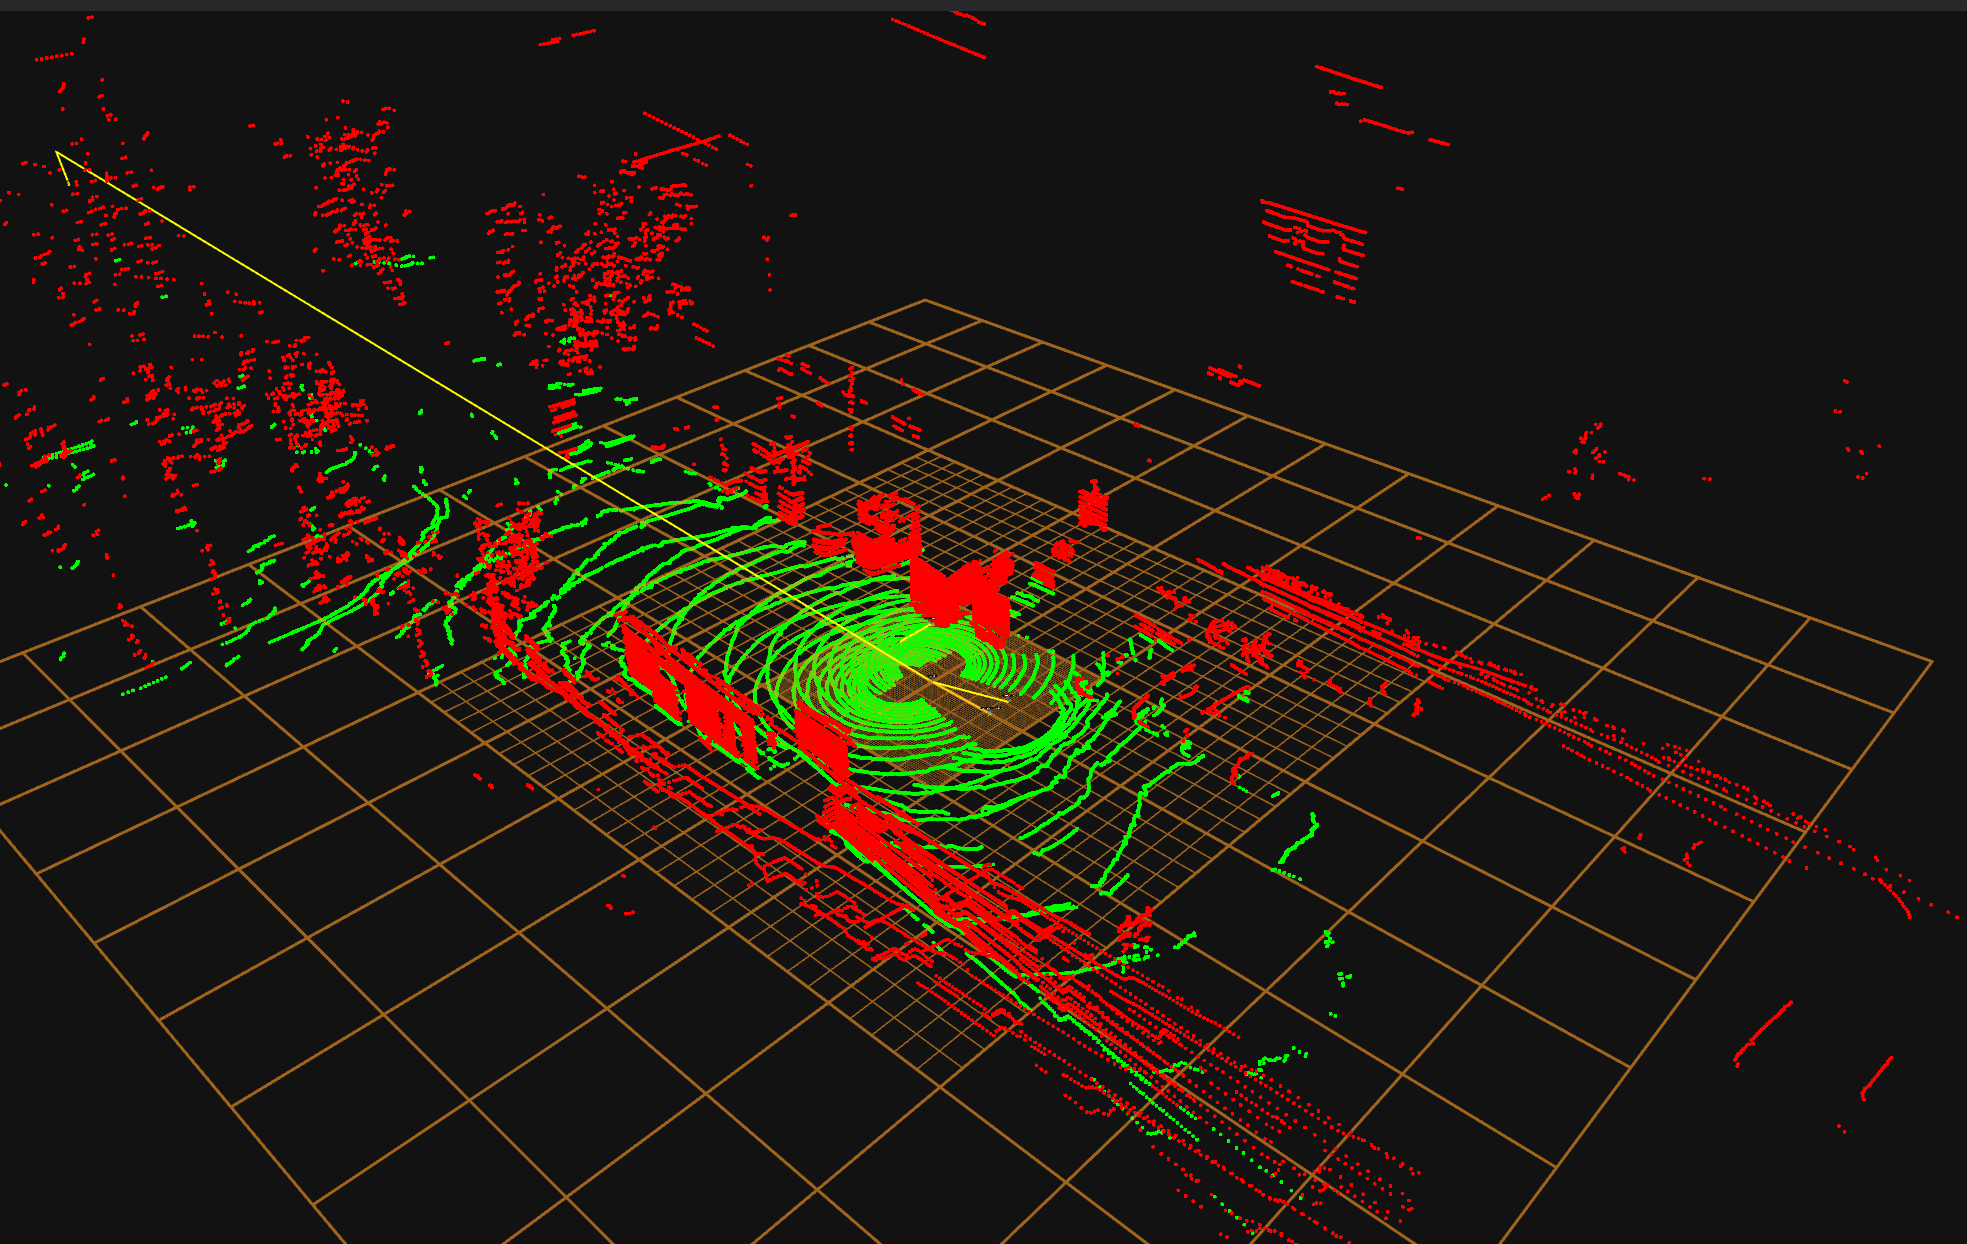
\includegraphics[width=\linewidth]{images/splitting_demo_pc} \\ а) Результат работы алгоритма.
	\end{minipage}
	\begin{minipage}[b][][b]{0.8\linewidth}\centering
		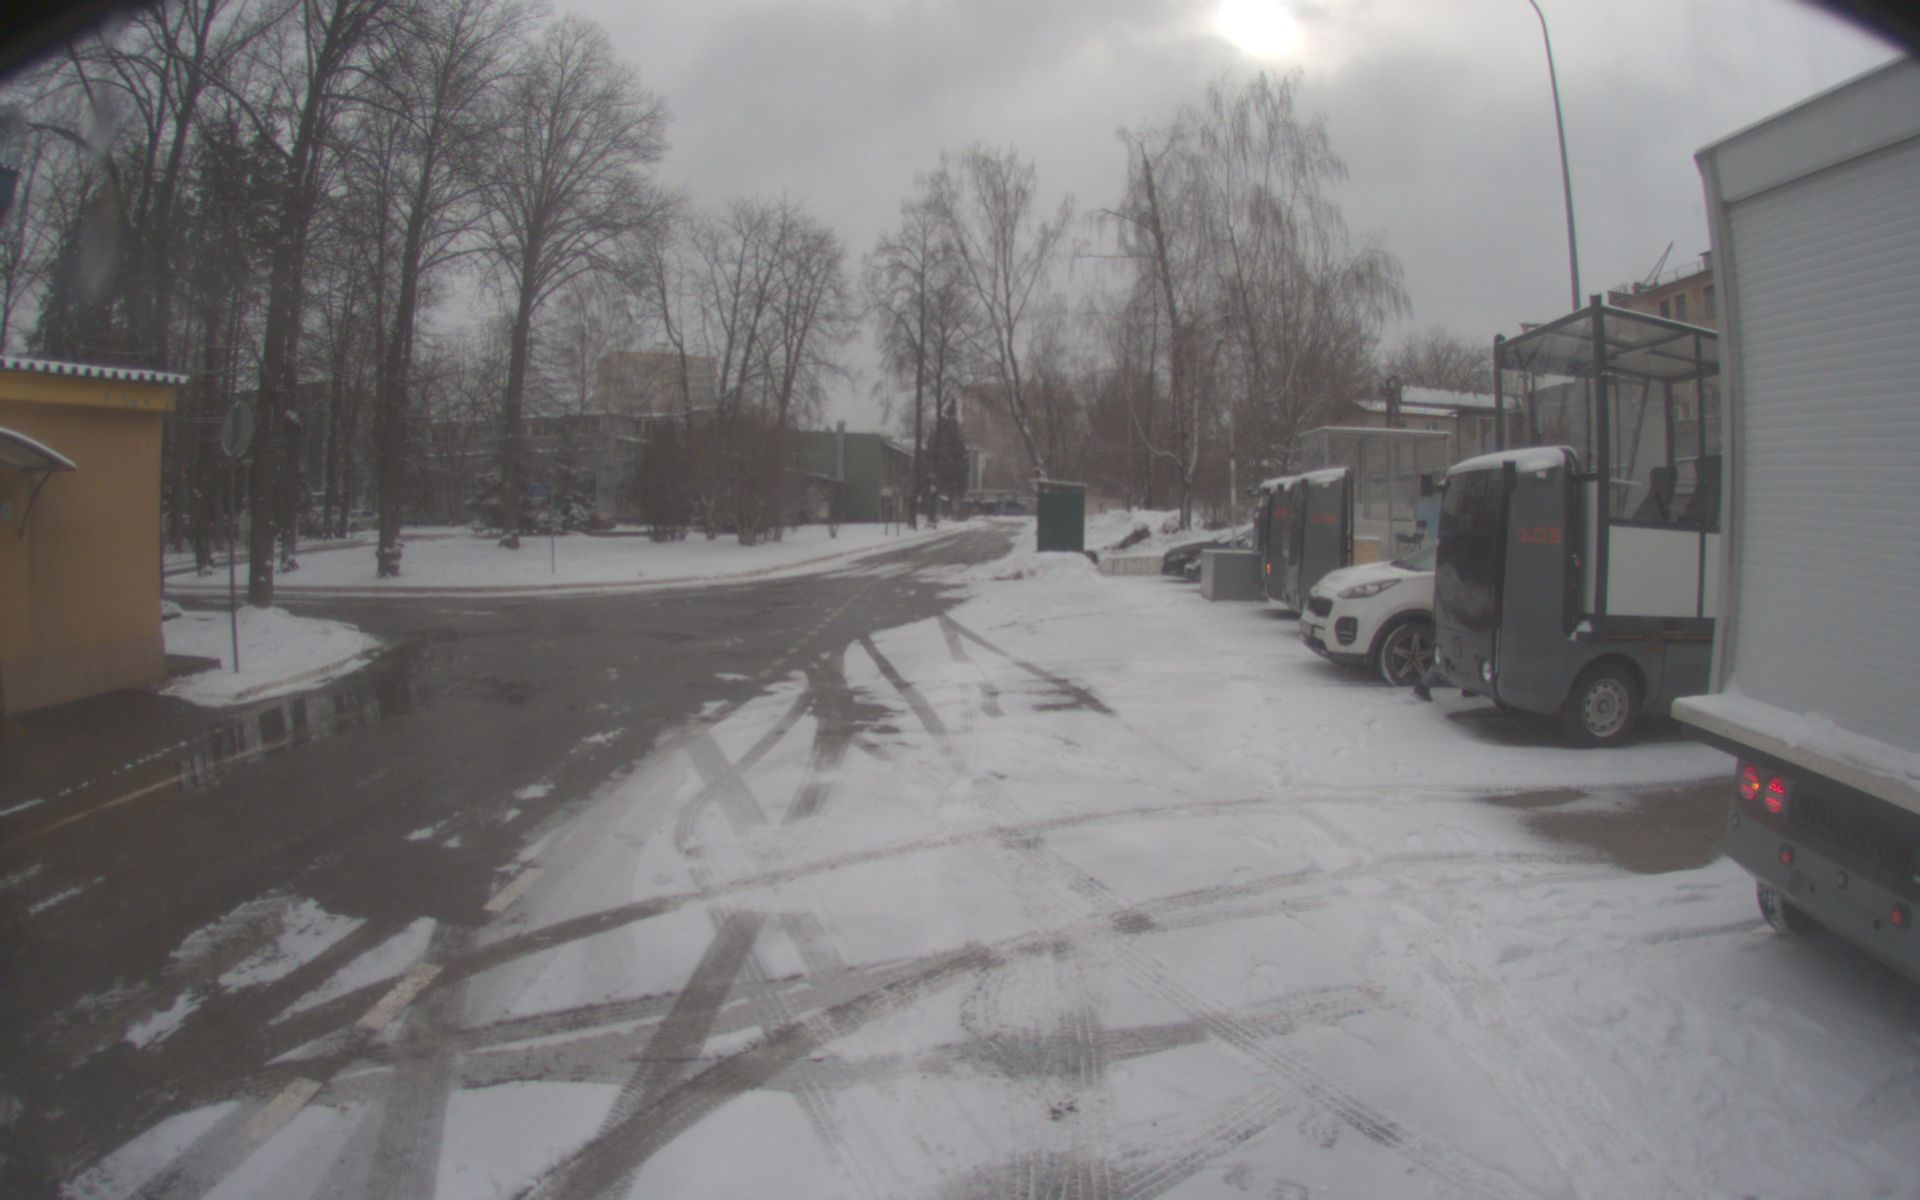
\includegraphics[width=\linewidth]{images/splitting_demo_img} \\ б) Изображение сцены с камеры БТС.
	\end{minipage}
	\hfill
	\caption{Пример работы алгоритма разделения облака точек земли и препятствий.}
	\label{fig:splitting_demo}
\end{figure}

Отметим, что данный алгоритм может быть реализован с помощью параллельных вычислений, в частности используя программно-аппаратную архитектуру CUDA, что позволяет снизить время выполнения данного алгоритма.

\section{Исследование эффективности алгоритма проекции визуальных детекций на основе комплексирования визуальных и лидарных данных}\label{sec:ch2/sec4}

Для оценки предложенного алгоритма~\ref{alg:true3ddet} было проведено его сравнение с подходами, не использующими комплексирование: с L-Shape алгоритмом, опирающимся только на визуальные данные, описанный в разделе~\cref{sec:ch2/sec1}, и с четырьмя алгоритмами вписывания в ориентированную рамку, разработанными для лидарных облаков точек.

\subsection{Описание эксперимента}

Эксперимент выполнялся на том же наборе данных, что и сравнение в разделе~\cref{sec:ch2/sec2}. Как и прежде, эталонными положениями объектов служили проекции аннотированных параллелепипедов на вид сверху, а для сравнения алгоритмов измерялся коэффициент Жаккара для сопоставленных вычисленных и эталонных повернутых ограничивающих рамок на виде сверху.

Отметим существенное отличие нового эксперимента от эксперимента в разделе~\cref{sec:ch2/sec2}. В последнем алгоритмы Rotating PCA, Diagonal PCA, Longest Diagonal и Rotated Triangle применялись к проекциям нижнего контура объектов, найденных на изображении, а не к выпуклым оболочками лидарных кластеров, как это было в оригинальной работе Ванга~\cite{Wang2021}. Данное ограничение использовалось поскольку в соответсвующем разделе исследовались алгоритмы, использующие исключительно визуальные данные. В новом же алгоритме из-за появления комплексирования с лидарными данными появляются лидарные кластеры (шаг~6 алгоритма~\ref{alg:true3ddet}), для работы с которыми и разрабатывались оригинальные алгоритмы. Поэтому в данном эксперименте перечисленные алгоритмы применялись к выпуклой оболочке получаемых лидарных кластеров, что отразится на полученных для них значениях коэффициент Жаккара в сравнении с результатами раздела~\cref{ch2/sec2}.

Как и ранее для сравниваемых алгоритмов было проведено исследование зависимости среднего коэффициента Жаккара от максимальной дистанции до детектируемых объектов.

Сравниваемые алгоритмы реализованы на языке Python. Помимо этого, предложенный алгоритм реализован на языке C++ в виде узла ROS (англ. Robot Operating System)~\cite{quigley2009ros} и интегрирован в систему управления БТС, что позволило проверить его применимость в режиме реального времени.

\subsection{Результаты экспериментов}

В таблице~\cref{tab:true3ddet-exp-res} приведены статистики измеренных коэффициентов Жаккара. Предложенный алгоритм комплексирования показывает средний коэффициент Жаккара $0.439$ против $0.337$ у L-Shape алгоритма, использующего только визуальные данные, что соответствует росту на $30.3$~\%. Лучший из подходов, использующих исключительно лидарные данные, -- Diagonal PCA -- достигает $0.399$, то есть предложенный алгоритм превосходит и его, примерно на $10$~\%.

\begin{table}[h!]
	\small
	\centering
	\begin{tabular}{|p{0.2\textwidth}|p{0.1\textwidth}|p{0.1\textwidth}|p{0.1\textwidth}|p{0.1\textwidth}|p{0.12\textwidth}|p{0.1\textwidth}|}
		\hline
		\textbf{Характеристика} & \textbf{Rotating PCA} & \textbf{Diagonal PCA} & \textbf{Longest Diagonal} & \textbf{Rotated Triangle} & \textbf{Предло\-женный} & \textbf{L-Shape}\\
		\hline
		\tiny Используемые\newline данные & \tiny лидар & \tiny лидар & \tiny лидар & \tiny лидар & \tiny лидар и камера & \tiny камера \\
		\hline
		Среднее & $0.396\newline(-9.8~\%)$ & $0.399\newline(-9.1~\%)$ & $0.335\newline(-23.7~\%)$ & $0.339\newline(-22.8~\%)$ & \boldmath$0.439\newline(-0.0~\%)$ & $0.337\newline(-23.2~\%)$ \\
		\hline
		\tiny Среднеквадратичное\newline отклонение & $0.222$ & $0.222$ & $0.188$ & $0.215$ & $0.256$ & \boldmath$0.141$ \\
		\hline
		Минимум & $0.008\newline(-89.7~\%)$ & $0.007\newline(-91.0~\%)$ & $0.004\newline(-94.9~\%)$ & $0.009\newline(-88.5~\%)$ & $0.004\newline(-94.9~\%)$ & \boldmath$0.078\newline(-0.0~\%)$ \\
		\hline
		$25$~\% & $0.212\newline(-7.8~\%)$ & $0.209\newline(-9.1~\%)$ & $0.187\newline(-18.7~\%)$ & $0.175\newline(-23.9~\%)$ & $0.219\newline(-4.8~\%)$ & \boldmath$0.230\newline(-0.0~\%)$ \\
		\hline
		$50$~\% & $0.400\newline(-5.4~\%)$ & $0.399\newline(-5.7~\%)$ & $0.331\newline(-21.7~\%)$ & $0.330\newline(-22.0~\%)$ & \boldmath$0.423\newline(-0.0~\%)$ & $0.328\newline(-22.5~\%)$ \\
		\hline
		$75$~\% & $0.562\newline(-13.8~\%)$ & $0.566\newline(-13.2~\%)$ & $0.457\newline(-29.9~\%)$ & $0.439\newline(-32.7~\%)$ & \boldmath$0.652\newline(-0.0~\%)$ & $0.451\newline(-30.8~\%)$ \\
		\hline
		Максимум & $0.872\newline(-5.7~\%)$ & $0.871\newline(-5.8~\%)$ & $0.734\newline(-20.6~\%)$ & $0.915\newline(-1.1~\%)$ & \boldmath$0.925\newline(-0.0~\%)$ & $0.736\newline(-20.4~\%)$ \\
		\hline
	\end{tabular}
	\caption{Статистики полученных коэффициентов Жаккара для предложено алгоритма и алгоритмов, не использующих комплексирование.}
	\label{tab:true3ddet-exp-res}
\end{table}

Вместе с тем по минимальному значению и по нижнему квартилю предложенный алгоритм уступает L-Shape алгоритму: $0.004$ против $0.078$ и $0.219$ против $0.230$ соответственно. Причина в том, что качество комплексирования зависит от количества лидарных точек, попавших на объект. Для удалённых либо существенно заслонённых объектов кластер вырождается в несколько точек, и построенная по нему рамка может грубо расходиться с эталоном. В то же время, L-Shape алгоритм строит рамку по проекции нижней границы объкта на плоскость движения с фиксированным количеством точек, что даёт устойчивую, хотя и невысокую в среднем, оценку. 

Зависимость среднего коэффициента Жаккара от ограничения дальности до детектируемых препятствий представлена на рис.~\cref{fig:true3ddet-metrics}. Предложенный алгоритм превосходит остальные во всём диапазоне рассмотренных дальностей. Кроме того, на графике видно, что предельная дальность, на которой алгоритмы, использующие лидарные данные, сохраняют работоспособность, более чем вдвое превышает соответствующую дальность для подхода, опирающегося только на визуальные данные.

\begin{figure}[ht!]
	\centering
	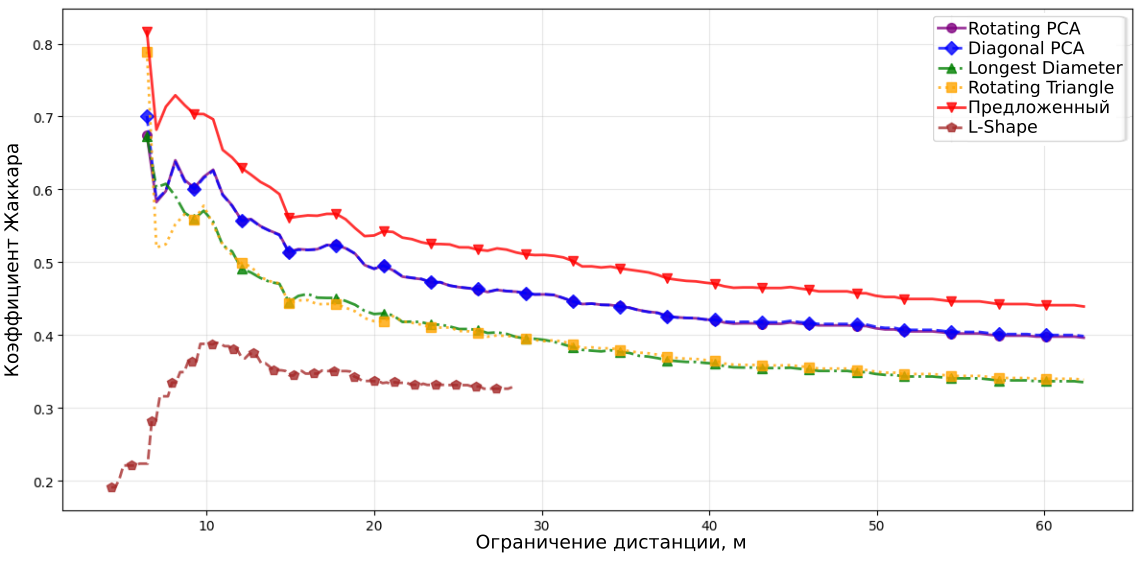
\includegraphics[width=\textwidth]{images/true3ddet_dist_plot.png}
	\caption{График зависимости среднего коэффициента Жаккара от ограничения дистанции до детектируемых препятствий для алгоритма комплексирования и алгоритмов, не использующих комплексирование.}
	\label{fig:true3ddet-metrics}
\end{figure}

\subsection{Вычислительная эффективность}

Измерение времени работы производилось для реализации предложенного алгоритма на языке C++ на вычислительной платформе с процессором AMD Ryzen 5 5600X, ОЗУ объёмом 32~Гб и ГПУ Nvidia GeForce RTX 3070. Среднее время обработки одного кадра составило $66.7$~мс при типичной частоте регистрации данных сенсорами БТС $10$~Гц, то есть при допустимом времени обработки в $100$~мс. Объём занимаемой памяти составил $178,8$~Мб ОЗУ и $156$~Мб памяти ГПУ. Полученные значения подтверждают применимость алгоритма на бортовом вычислителе БТС в режиме реального времени.

Время отдельных этапов алгоритма, измеренных с помощью библиотеки инструментального профилироввания Tracy~\cite{kyostila2008tracy}, приведено на рис~\cref{fig:true3ddet-perf}. Основную долю времени занимают шаги~4 и~5 алгоритма~\ref{alg:true3ddet}, в которых в текущей реализации дважды выполняется проецирование точек кластеров на плоскость изображения с коррекцией дисторсии. Эта операция выполняется на ЦПУ, хотя, как отмечено в разделе~\cref{sec:ch2/sec3}, хорошо поддаётся распараллеливанию на ГПУ, что оставляет запас для дальнейшей оптимизации.

\begin{figure}[ht]
	\centering
	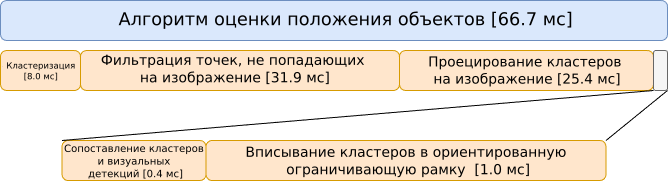
\includegraphics[width=0.6\textwidth]{images/True3DPerf.png}
	\caption{Среднее время выполнения этапов алгоритма~\ref{alg:true3ddet}}
	\label{fig:true3ddet-perf}
\end{figure}

\section{Алгоритм проекции сегментации проезжей части на изображении на плоскость движения ТС}\label{sec:ch2/sec5}

Помимо определения положения препятствий в окружающей БТС сцене важную роль в осуществлении безопасного решения задач планирования пути играет включение в модель описание областей свободных для перемещения БТС. Это позволяет алгоритмам планирования пути различать области, для которых достоверно известно отсутствие в нём каких либо объектов, от областей, для которых отсутствует информация, позволяющая судить о его проходимости ввиду окклюзии либо недостоверности регистрируемых данных. На Рисунке~\cref{fig:occlusion} привидён пример, демонстрирующий важность этого различия. Мы можем обучить нейросетевую модель YOLOP или другую модель, осуществляющую семантическую сегментацию двумерных изображений, сегментировать проезжую часть на изображении. Однако аналогично задаче проецирования препятствий в трехмерную систему координат БТС $O_l$, описанной в разделе~\cref{sec:ch2/sec1}, мы столкнёмся с необходимостью спроецировать полученную сегментацию на вид сверху. В данном разделе предложен алгоритм, осуществляющий данное проецирование на основе комплексирования данных с камеры и лидаров, установленных на БТС. Дополнительно будет предложена модификация алгоритма, позволяющая добавлять при проецировании области, содержащие некрупные препятствия.

\begin{figure}[ht!]
	\centering
	\begin{minipage}[b][][b]{0.49\linewidth}\centering
		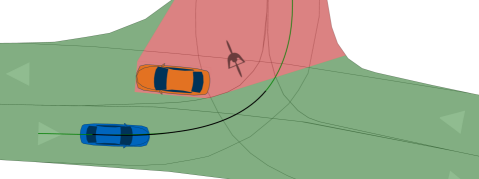
\includegraphics[width=\linewidth]{images/occlusion_a} \\ а) БТС (синий) не видит велосипедиста позади автомобиля. Зелёным выделена территория в поле видимости датчиков БТС, красным -- области, о которых нет информации ввиду их окклюзии
	\end{minipage}
	\begin{minipage}[b][][b]{0.49\linewidth}\centering
		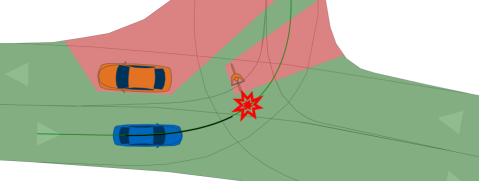
\includegraphics[width=\linewidth]{images/occlusion_b} \\ б) При продолжении движения велосипедист детектируется датчиками БТС, но из-за близости объекта, у систем управления остаётся мало времени для реагирования.
	\end{minipage}
	\hfill
	\caption{Демонстрация влияния окклюзии на безопасность движения БТС~\cite{Moller2024}.}
	\label{fig:occlusion}
\end{figure}

В отличие от типичных препятствий в окружающей БТС сцене: людей, автомобилей; размеры и положение которых с высокой точностью описываются ориентированными ограничивающими рамками, проезжая часть после проекции имеет сложную геометрию (рисунок~\cref{fig:road_segmentation}). Из-за этого векторное представление проезжей части на виде сверху может быть неудобным для построения. Вместо него мы воспользуемся представлением в виде сетки, фиксированного разрешения, где каждому элементу будет сопоставлен класс <<свободно>> -- в случае если в соответствующей области БТС может безопасно проезжать, или <<неизвестно>> -- в случае если информации об области недостаточно (а далее и дополнительный класс <<занято>> для областей, где обнаружен объект).

\begin{figure}[ht]
	\centering
	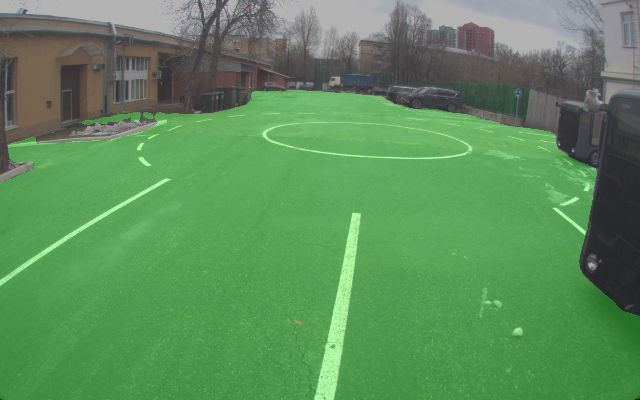
\includegraphics[width=0.7\textwidth]{images/road_segmentation}
	\caption{Пример семантической сегментации проезжей части моделью YOLO на изображении с камеры БТС.}
	\label{fig:road_segmentation}
\end{figure}

Прежде чем приступить к описанию алгоритма опишем интуицию, которая будет лежать в его основе без использования информации с лидаров. Воспользуемся предположением в наивном подходе проецирования препятствий из раздела~\cref{sec:ch2/sec1} о совпадении поверхности дорожной части с плоскотью $z_l = 0$. В такой модели оценка проходимости элемента сводится к проекции центров сетки на плоскость изображения(как и прежде мы считаем внутреннюю и внешнюю калибровки камеры известными), если при проецировании центр элемента попал на пиксель, классифицированный как проезжая часть -- соответствующий элемент сетки классифицируется <<свободным>>,в противном случае <<неизвестно>> (рисунок~\cref{fig:plane_proj}). Отметим, что в последнем случае нельзя утверждать, что область не свободна для проезда, т.к. она может быть заслонена другим объектом -- см. рисунок~\cref{fig:human_shadow}). Листинг~\ref{alg:naive_true3dsegm} приводит описание данного алгоритма.

\begin{algorithm}
	\caption{Алгоритм проецирования проезжей части на вид сверху (наивный).}
	\label{alg:naive_true3dsegm}
	\LinesNumbered
	\KwIn{$S_I$ -- семантическая сегментация проезжей части на изображении $I$; $\text{res}$ -- разрешение сетки[пикс/м], на которую производится проецирование; $l$ -- ширина и высота сетки[м]}
	\KwOut{$S_{BEV}$ -- проекция сегментации проезжей части на вид сверху}
	$s \leftarrow \dfrac{1}{\text{res}}$ \;
	$L \leftarrow l \cdot \text{res}$ \;
	$S_{BEV} \leftarrow $ матрица размера $L\times L$\;
	\For{$i \leftarrow 0$ \KwTo $L$}{
		\For{$j \leftarrow 0$ \KwTo $L$}{
			$x \leftarrow -\dfrac{l}{2} + js$\;
			$y \leftarrow -\dfrac{l}{2} + is$\;
			$(u;v) \leftarrow$ проекция $(x,y,0)$ на изображение (с учётом дисторсии)\;
			\eIf{$(u,v)$ попадает на изображение AND $S_I[u][v] ==$ <<свободно>>}{
				$S_{BEV}[u][v] \leftarrow$ <<свободно>>\;
			}{
			    $S_{BEV}[u][v] \leftarrow$ <<неизвестно>>\;
			}
		}
	}
   \Return{$S_{BEV}$}\;
\end{algorithm}

\begin{figure}[ht]
	\centering
	\includegraphics[width=0.8\textwidth]{images/PlaneProj}
	\caption{Иллюстрация алгоритма проецирования в сценарии, когда проезжая часть лежит в известной плоскости. Для облегчения восприятия проецируемая сетка представлена одним рядом.}
	\label{fig:plane_proj}
\end{figure}

\begin{figure}[ht]
	\centering
	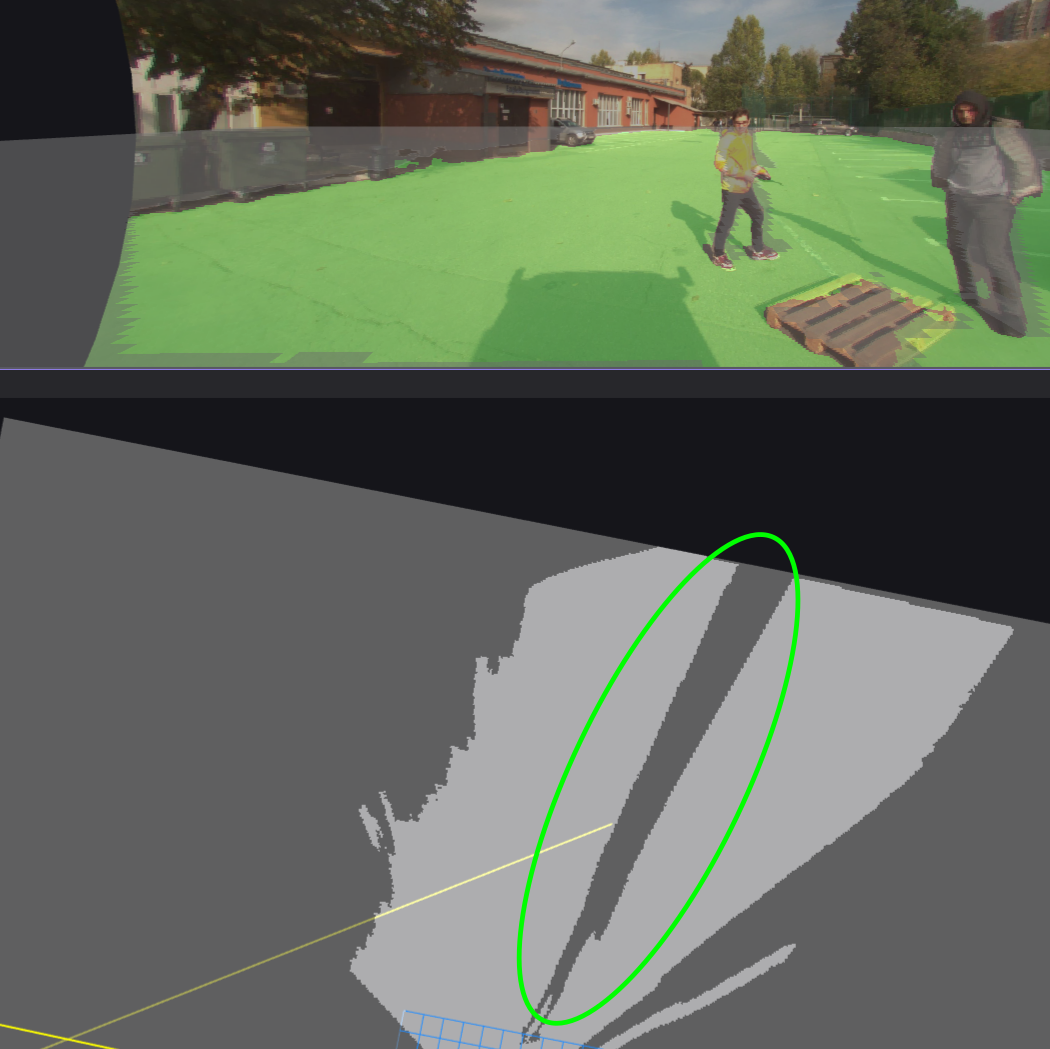
\includegraphics[width=0.7\textwidth]{images/human_shadow_segmentation}
	\caption{Пример заслонённой области свободной для проезда.}
	\label{fig:human_shadow}
\end{figure}

Однако, мы уже показали низкое качество моделей, использующих предположение о совпадении поверхности проезжей части с плоскостью. Ослабим это предположение и обобщим алгоритм на этот случай. Будем считать, что поверхность описывается некоторой известной функцией $z_l = z(x_l, y_l)$. Тогда в ранее описанный алгоритм достаточно добавить вычисление этой координаты перед проецированием на изображение(Листинг~\ref{alg:gen_true3dsegm}). На рисунке~\cref{fig:non_plane_proj} представлена иллюстрация обобщённого алгоритма. Очевидно, для корректной работы алгоритма необходимо, чтобы более близкие к БТС участки проезжей части не перекрывали обзор камеры для более удалённых участков. При достаточной гладкости проезжей части, разумном разрешении итоговой сетки на виде сверху и достаточной высоте расположения камеры, это требование будет выполняться.

\begin{algorithm}
	\caption{Обобщение алгоритма проецирования проезжей части на вид сверху.}
	\label{alg:gen_true3dsegm}
	\LinesNumbered
    Аналогично шагам 1--7 из Листинга~\ref{alg:naive_true3dsegm}\;
			$(u;v) \leftarrow$ проекция $(x,y,z(x,y))$ на изображение (с учётом дисторсии)\;
	Аналогично шагам 9--16 из Листинга~\ref{alg:naive_true3dsegm}\;	
\end{algorithm}

\begin{figure}[!h]
	\centering
	\includegraphics[width=0.8\textwidth]{images/NonPlaneProj}
	\caption{Иллюстрация алгоритма проецирования в сценарии, когда поверхность проезжей части удовлетворяет уравнению $z=z(x,y)$. Для облегчения восприятия проецируемая сетка представлена одним рядом.}
	\label{fig:non_plane_proj}
\end{figure}

\subsection{Вычисление функции $z(x,y)$.}\label{sec:ch2/ground_height_estimation}

Для завершения разработки алгоритма необходимо предложить способ оценить значения $z(x,y)$ в центрах сетки, на которую производится проекция сегментации. Для этого аналогично разделу~\cref{sec:ch2/sec3} мы воспользуемся комплексированием данных, зарегистрированными лидарами. Как и прежде мы будем считать, что облака точек с лидаров прошли предварительную обработку и представлены единым облаком точек с компенсированным движением БТС во время регистрации облаков. Для дальнейшего вычисления $z(x,y)$ предложим два подхода:

\begin{enumerate}
	\item \textbf{Использовать облако точек земли, полученных алгоритмом~\ref{alg:pc_splitting}}. В этом случае облако вычисляются прямоугольные проекции на сетку. За $z$ тех элементов сетки, в которых оказалась проекции точек, берётся среднее, минимум, максимум или произвольное из координат $z$ этих точек. Для оставшихся не инициализированных точек необходимо произвести триангуляцию точек попавших на сетку. Далее для каждой точки сетки находится треугольник, содержащий её. Высота анализируемой точки получается путём линейной интерполяции. Пусть $v_1, v_2, v_3$ -- вершины выбранного треугольника на виде сверху, $z_1, z_2, z_3$ -- координата $z$ этих вершин соответственно. Пусть вершина $v$, координата $z$ которой интерполируется, образует с вершинами выбранного треугольника три треугольника площадью $S_1, S_2, S_3$. Тогда искомая координата вычисляется по формуле: $z=\dfrac{z_1S_1 + z_2S_2 + z_3S_3}{S_1+S_2+S_3}$~\cite{PhysRevB.63.045120} (рисунок~\cref{fig:z_interpolation}). В качестве триангуляции используется триангуляция Делоне~\cite{leach1992improving}. По определению, при такой триангуляции треугольники обладают тем свойством, что описанные вокруг них окружности не содержат других триангулируемых точек. Поскольку лидарные точки земли по принципу работы датчика  образуют приближённо набор дуг (так называемых <<колец>>), это свойство гарантирует, что интерполяция будет происходить по точкам, принадлежащим разным кольцам, что делает её более точной. Рисунок~\cref{fig:whydelaunay} демонстрирует разницу в выборе интерполируемых трёх точек при триангуляции Делоне и трёх ближайших соседей.
	
	\item \textbf{Добавить в алгоритм~\ref{alg:pc_splitting} дополнительные тестовые точки.} В качестве этих точек будут выступать центры искомой сетки. Недостатком такого подхода станет увеличение времени работы алгоритма~\ref{alg:pc_splitting}, что замедлит время обработки алгоритмы, использующие его результаты, в частности, алгоритма~\ref{alg:true3ddet}. Однако при наличии вычислительных ресурсов на ГПУ вычисление регрессии можно расспараллелить с использованием механизма мультипоточности CUDA Streams~\cite{Rennich}. В этом случае в регрессии можно переиспользовать матрицу $K$ из уравнения~\cref{eq:cov_gpr}. Затем вычислить ковариационные матрицы $\widetilde{K_*}, \widetilde{K_{**}}$ для новых тестовых точек, и аналогично~\cref{eq:gpr_predict} вычислить аппроксимацию $z$ в тестовых точках. На рисунке~\cref{fig:nsys_splitting_streams} представлены результаты профилирования ресурсов на ГПУ с помощью Nsight Systems~\cite{nsight-systems_2025} изменившейся части программы, реализующей алгоритм~\ref{alg:pc_splitting} при последовательном  и параллельном решении задач регресии. Программа реализована на языках C++ и CUDA C++. Профилирование происходило на ПК с процессором AMD Ryzen 5 5600X с 6~ядрами и тактовой частотой 4,6~ГГц, ОЗУ объёмом 32~Гб, а также ГПУ Nvidia GeForce 3070 с графической памятью 8~Гб и тактовой частотой 1,5~ГГц. Количество основных точек составило порядка 100~000 точек, количество дополнительных точек составило 10~000. На рисунке~\cref{fig:splitting_with_streams} представлен график сравнения распределения времени работы алгоритма разделения при последовательном и параллельном вычислениях. 
\end{enumerate}

\begin{figure}[ht]
	\centering
	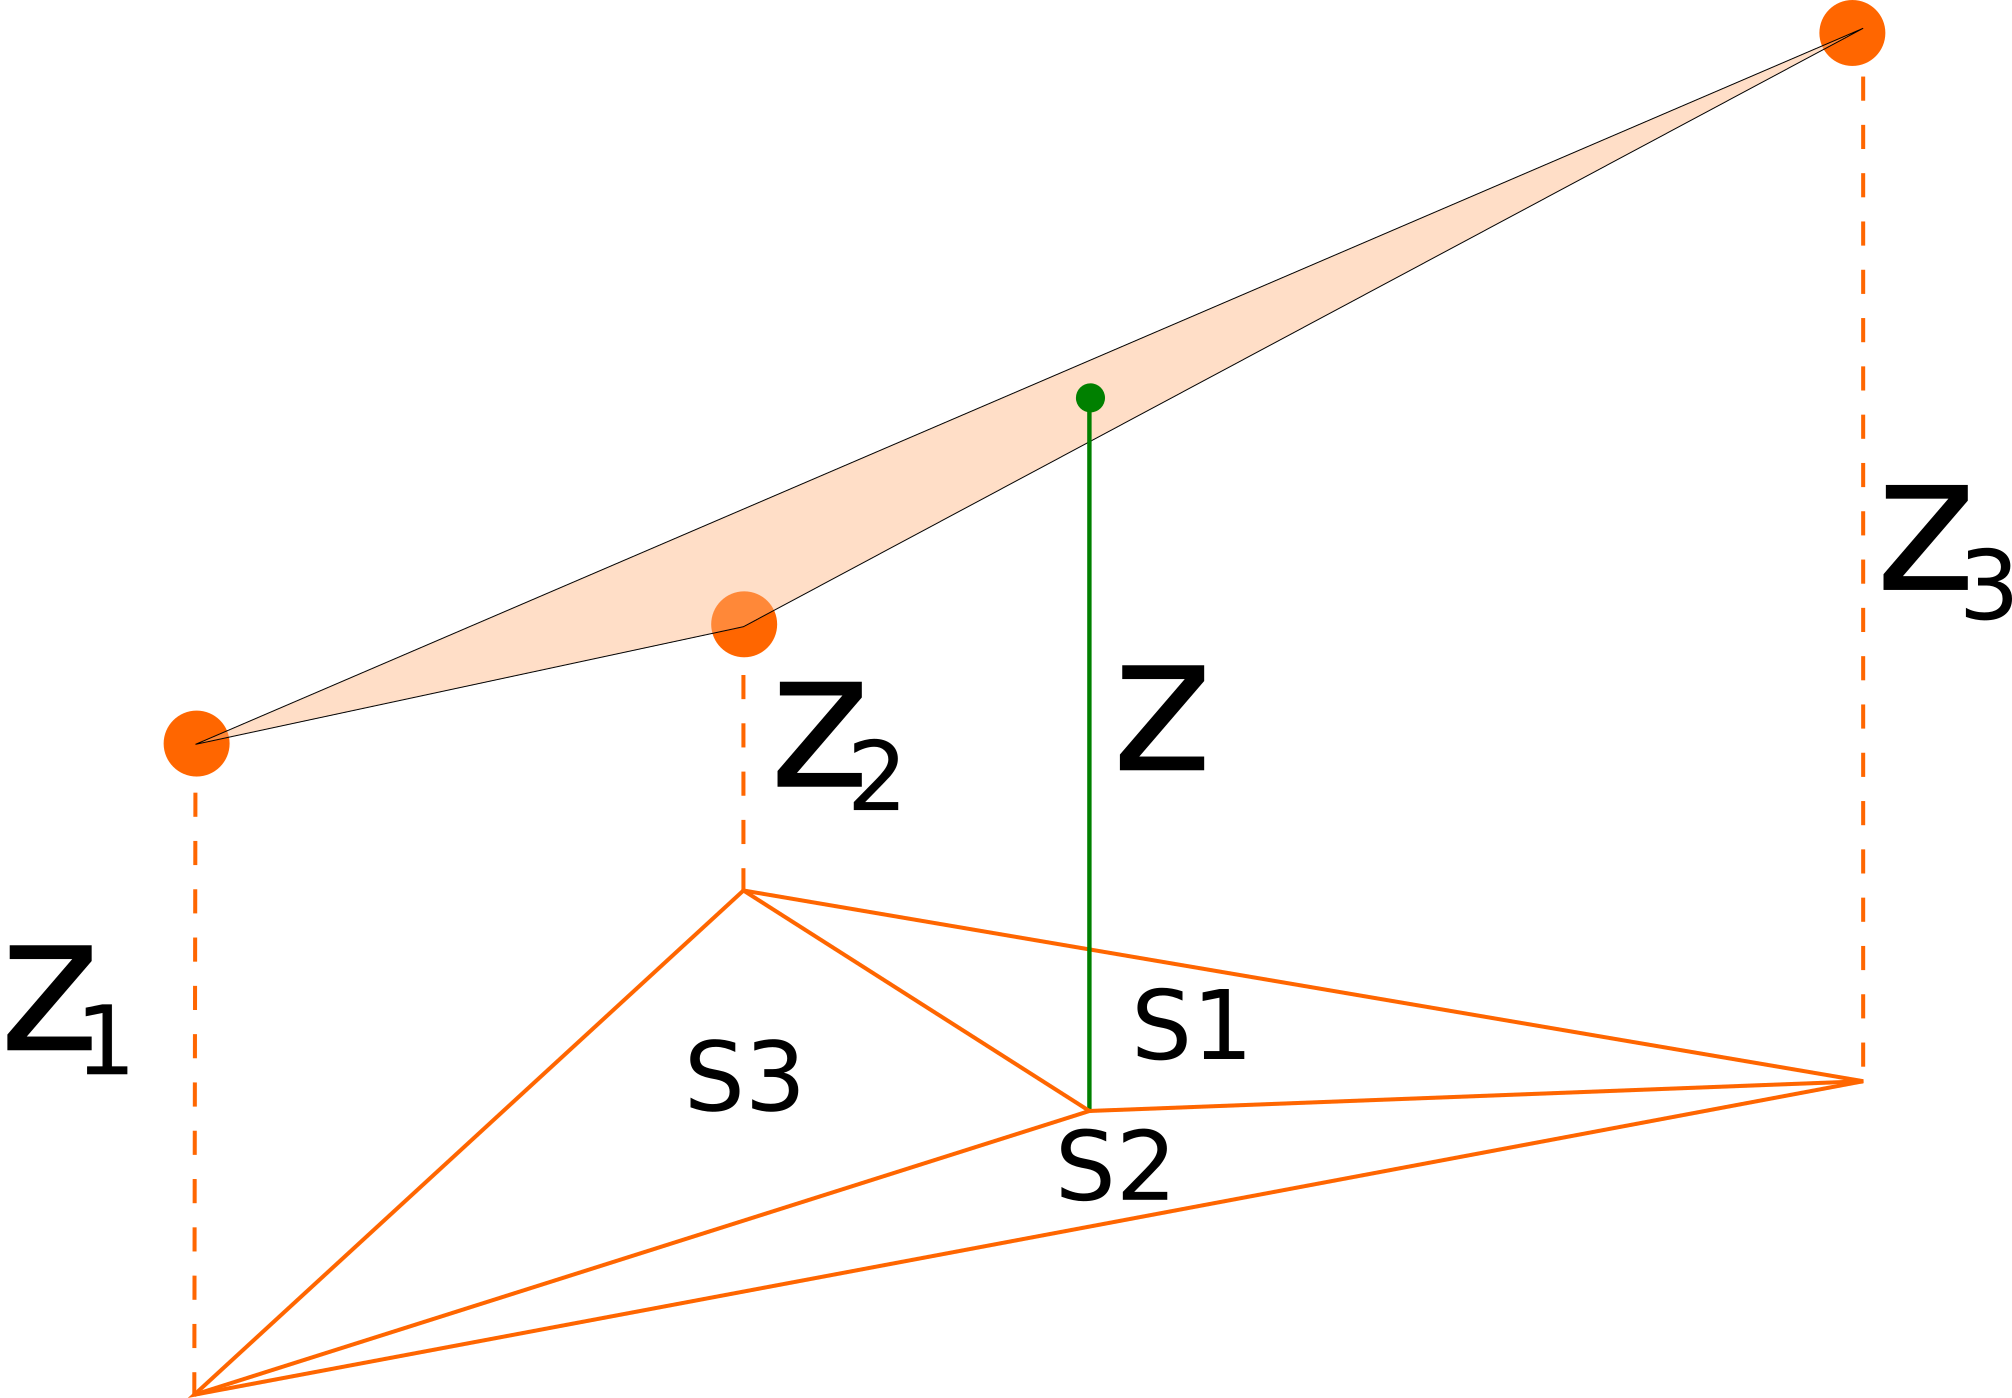
\includegraphics[width=0.6\textwidth]{images/z_interpolation}
	\caption{Линейная интерполяция $z$ в треугольнике.}
	\label{fig:z_interpolation}
\end{figure}


\begin{figure}[ht]
	\centering
	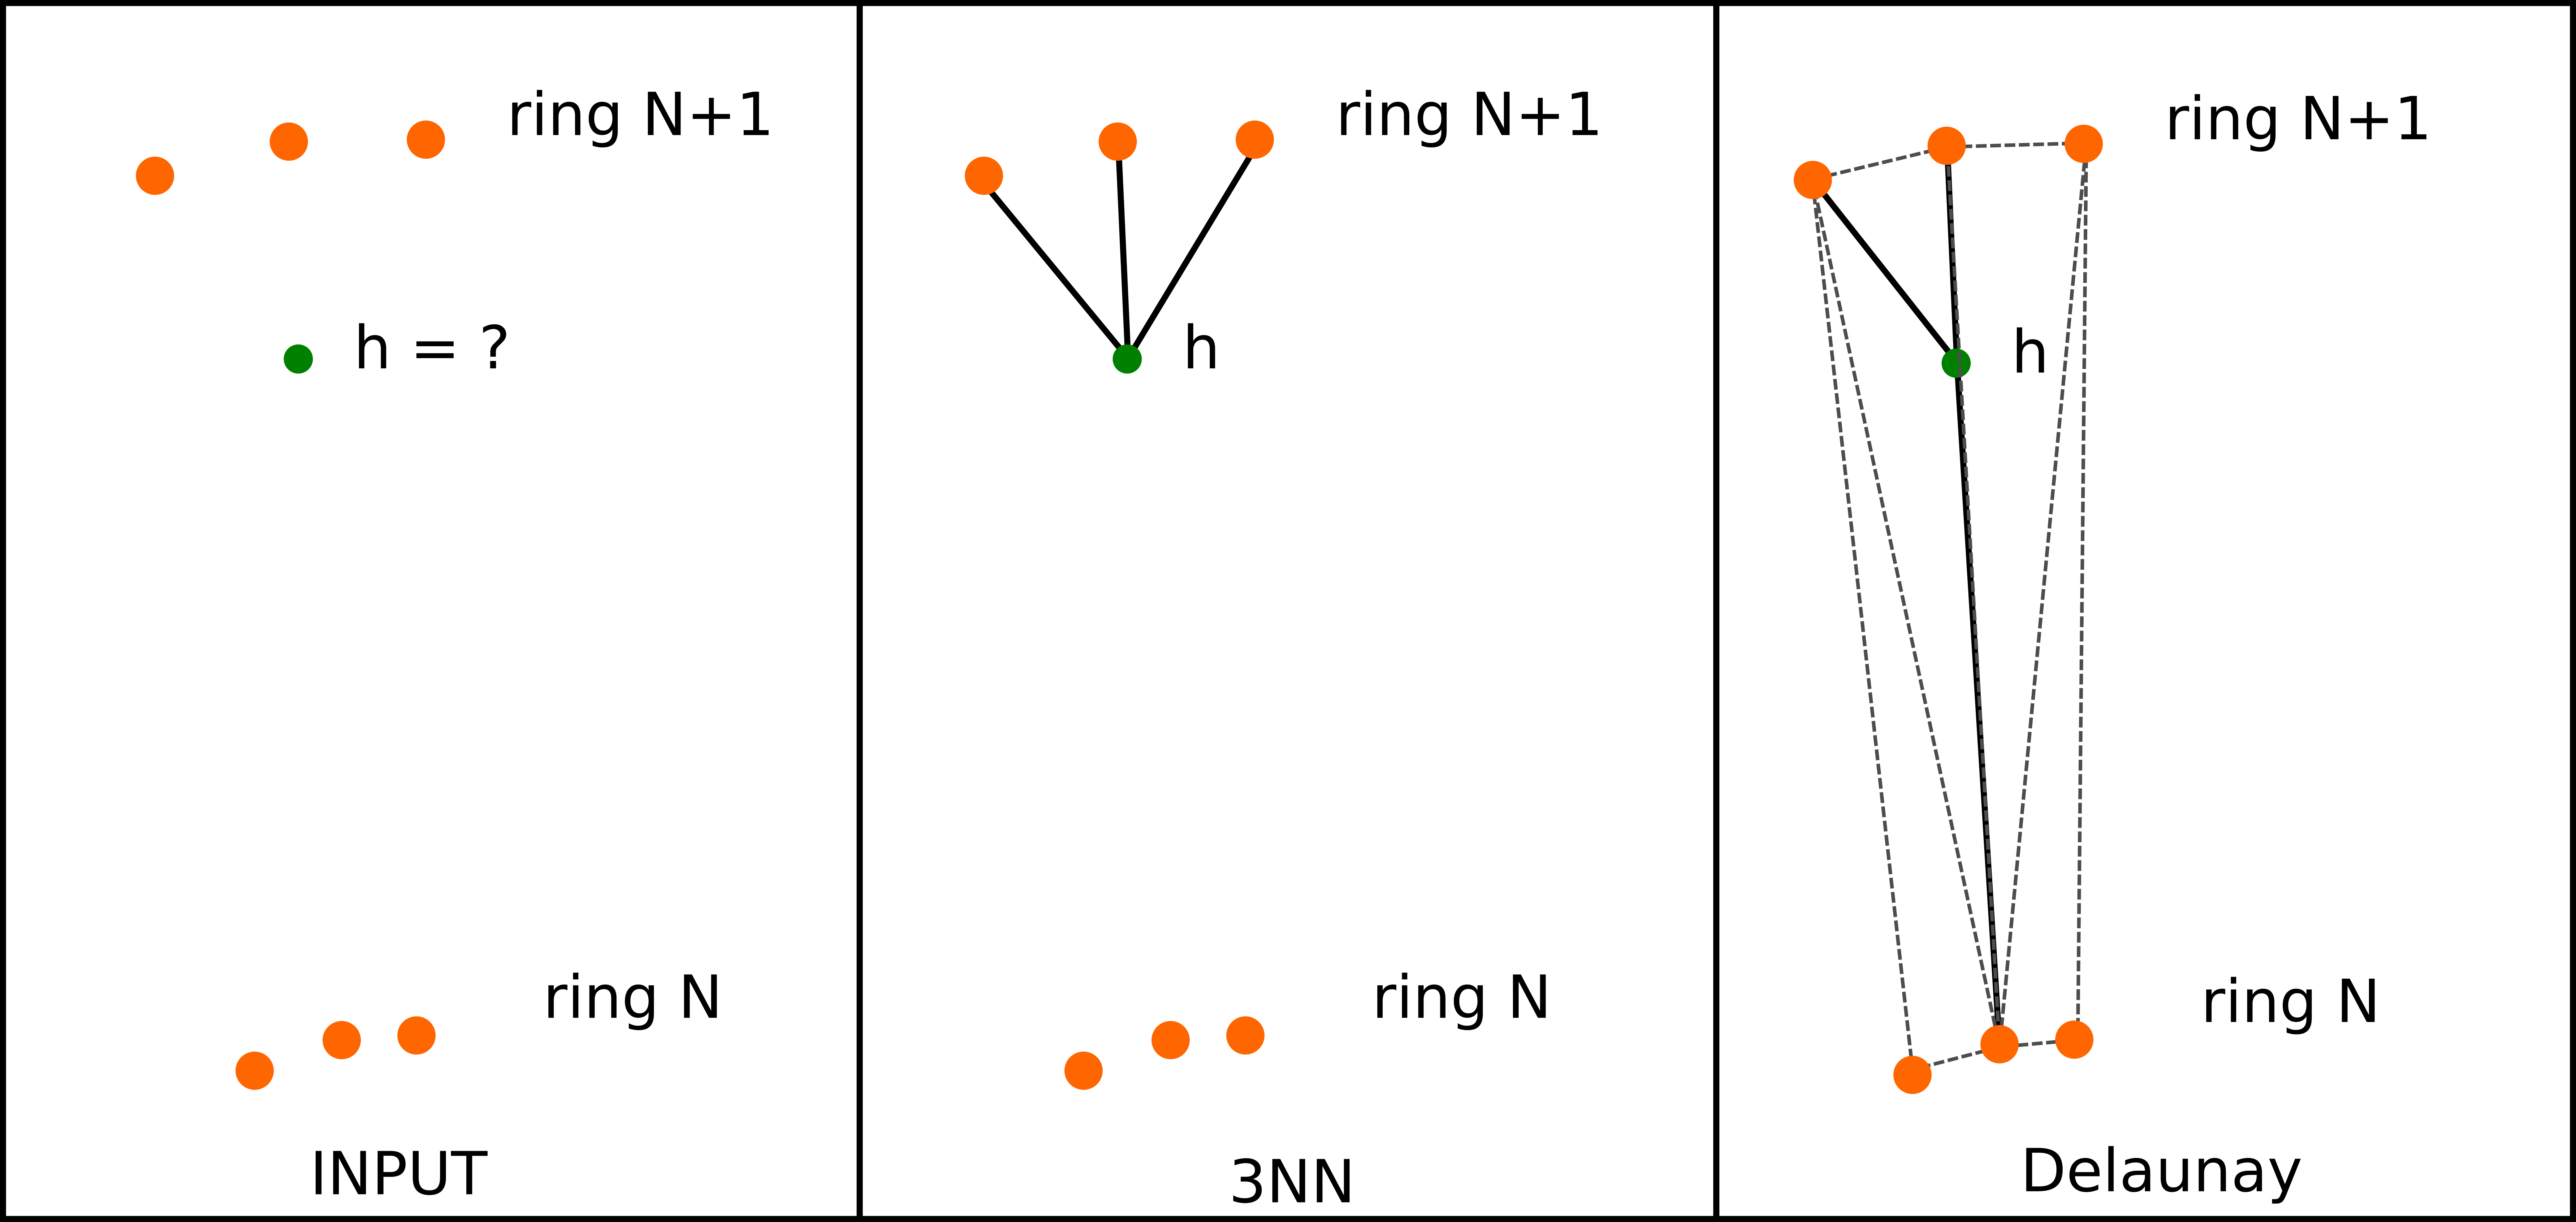
\includegraphics[width=0.6\textwidth]{images/whydelaunay}
	\caption{Мотивация использования триангуляции Делоне.}
	\label{fig:whydelaunay}
\end{figure}

\begin{figure}[ht]
	\begin{minipage}[b][][b]{\textwidth}\centering
		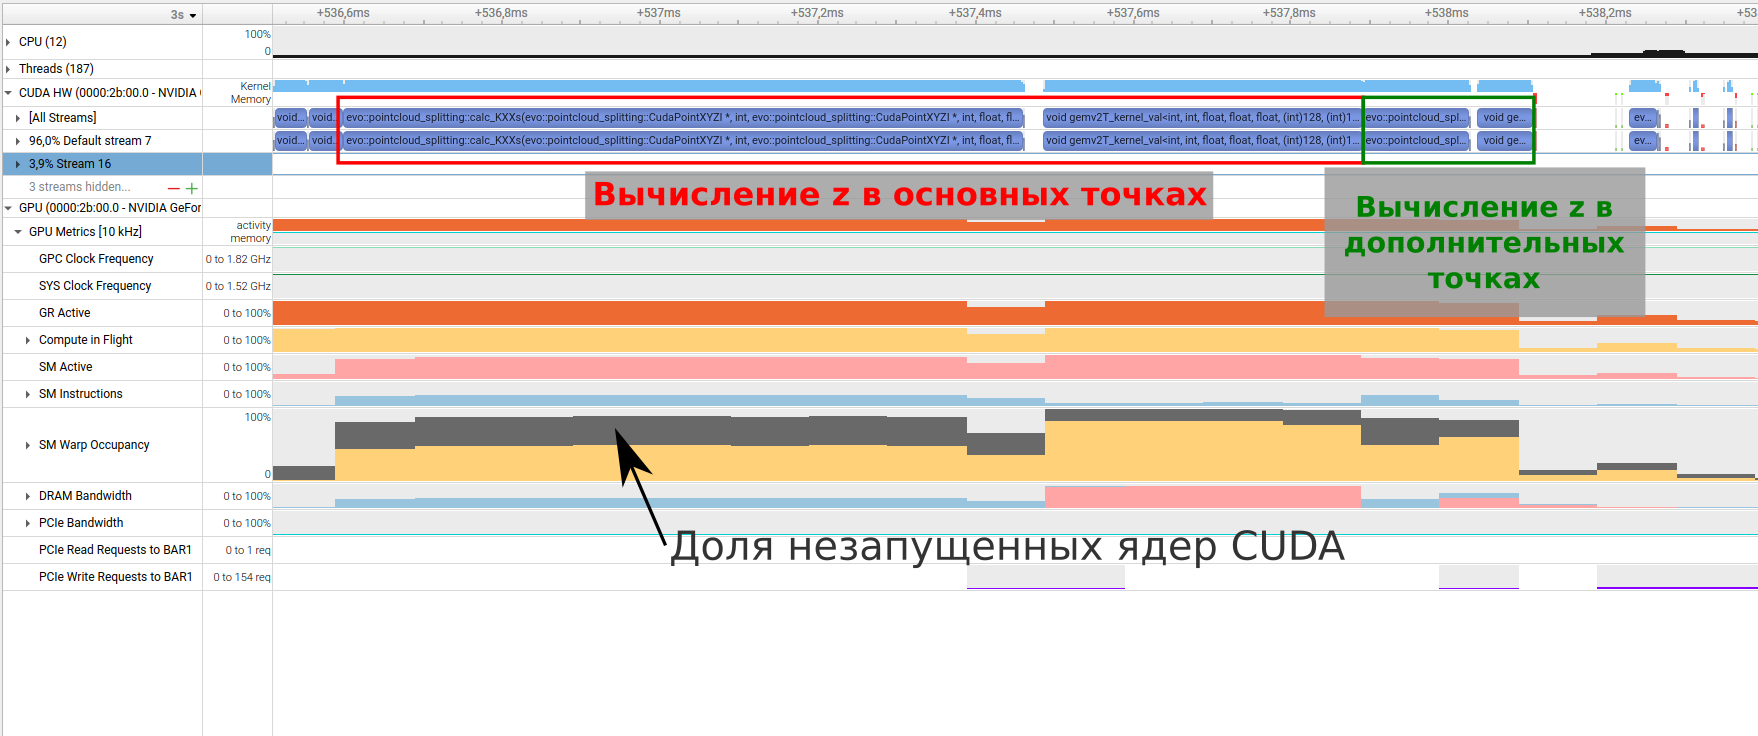
\includegraphics[width=\textwidth]{images/nsys_splitting_wo_streams} \\ а) Без использования CUDA Streams
	\end{minipage}
	\hfill
	\begin{minipage}[b][][b]{\textwidth}\centering
		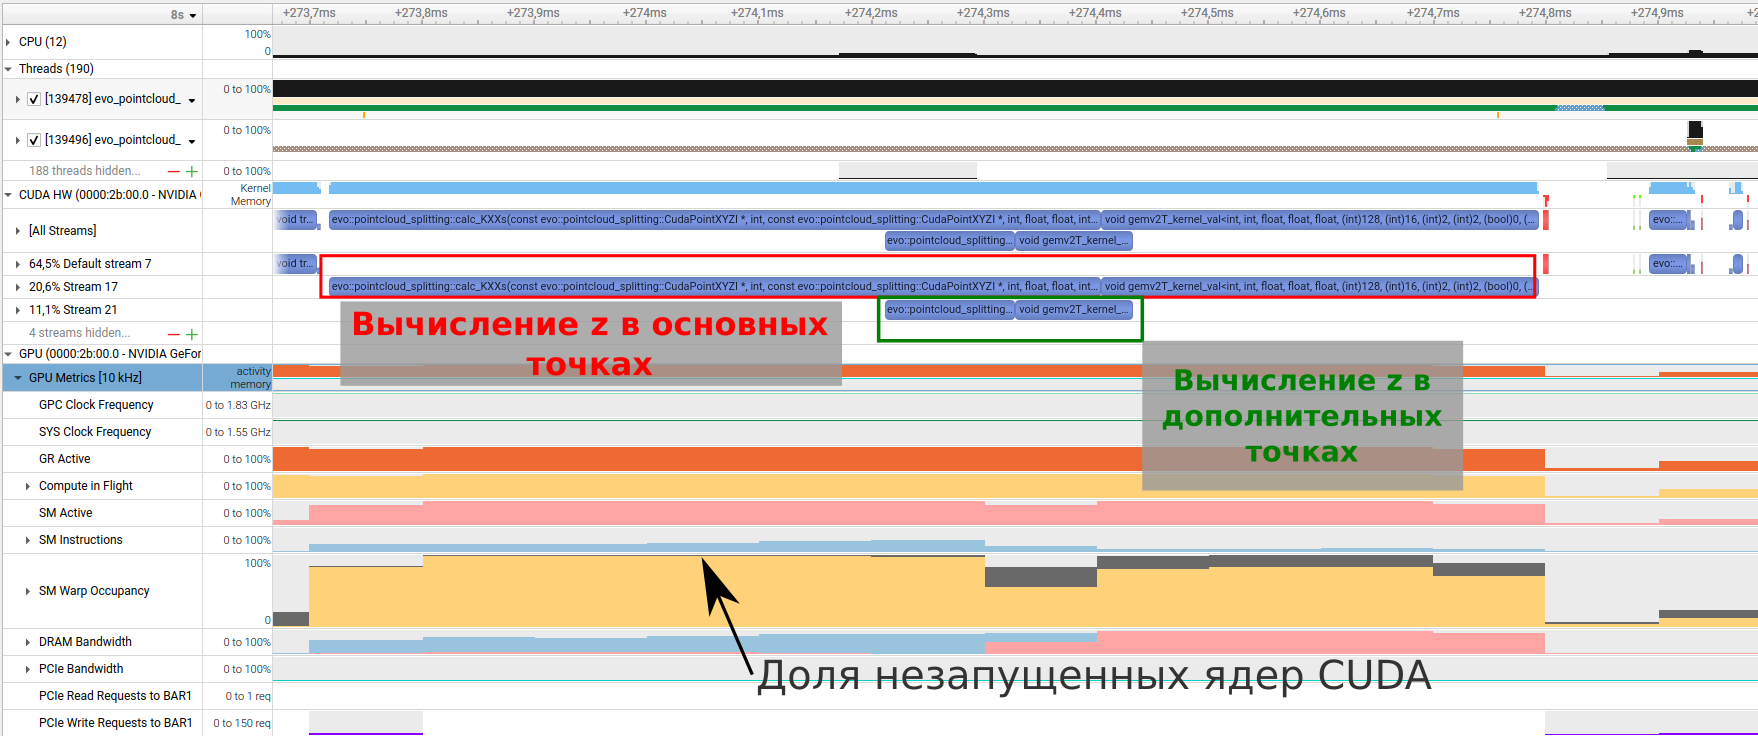
\includegraphics[width=\textwidth]{images/nsys_splitting_with_streams} \\ б) С исправленной конфигурацией запуска ядер CUDA и использование CUDA Streams
	\end{minipage}
	\legend{Красной рамкой выделены вычисления аппроксимации прежних тестовых точек, в зелёной -- дополнительных точек. Во вкладке <<SM Warp Occupancy>> жёлтым показана доля вычисляемых ядер относительно максимальной теоретической пропускной способности архитектуры в данный момент времени, серым -- доля ядер, которым не хватило ресурсов для вычисления и в результате простаивающих в ожидании их появления.}
	\caption{Профилирование в Nsight Systems изменившейся части программы, реализующей алгоритм~\ref{alg:pc_splitting}, при добавлении дополнительных точек для аппроксимации. }\label{fig:nsys_splitting_streams}
\end{figure}

\begin{figure}[ht]
	\centering
	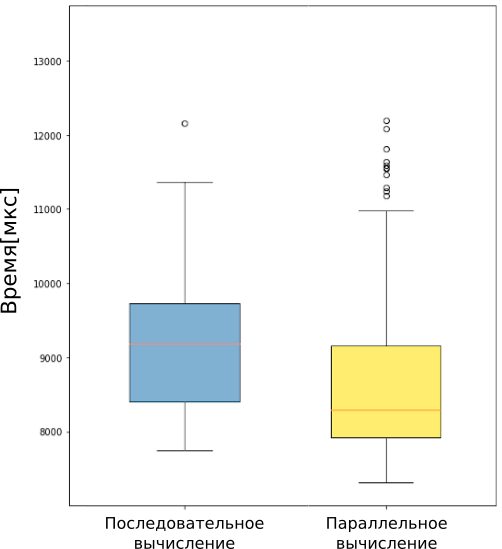
\includegraphics[width=0.6\textwidth]{images/splitting_with_streams}
	\caption{График полного времени работы алгоритма~\ref{alg:pc_splitting} с дополнительными тестовыми точками при последовательном и параллельном вычислении.}
	\label{fig:splitting_with_streams}
\end{figure}


Отметим, что второй подход возможно реализовать с использованием параллельных вычислений средствами CUDA: т.к. после регрессии на основе гауссовских процессов каждый элемент сетки, на который проецируется сегментация обрабатывается независимо от других элементов. В то же время первый подход требует произвести триангуляцию Делоне, для которой реализации на ГПУ существуют~\cite{rong2008computing}, но эксперименты с данной реализацией показали замедление алгоритма на $10$~мс или $20$~\% в сравнении с реализацией на ЦПУ, которая занимает в среднем $50$~мс.

\subsection{Модификация алгоритма для обнаружения препятствий на проезжей части}

В разделе~\cref{sec:ch2/sec3} был представлен алгоритм оценки положения детекций на изображении в трехмерной системе координат БТС $O_l$. Ограничением этого алгоритма является необходимость алгоритма детекции объектов быть обученным на распознование конкретных типов объектов. Как правило, такие модели способны надёжно распознавать людей, машин, животных, дорожные знаки. Однако многие типы объектов в реальном мире встречаются редко либо их объекты сильно различаются между собой  из-за чего обучение модели для них представляется возможным ввиду малого размера обучающей выборки. В то же время в контексте решаемой нами задачи можно заметить, что проезжая часть редко содержит <<вырезы>> малого размера особенно на пути следования БТС. Воспользовавшись этим предположением можно модифицировать алгоритм~\ref{alg:gen_true3dsegm}: после завершения проецирования сегментации на вид сверху произвести поиск замкнутых областей, классифицированных как <<неизвестно>> внутри полученной проекции, площадью в некотором интервале $\left[a_{low}, a_{high}\right]$ и задать им новый класс <<занято>> (Листинг~\ref{alg:true3dsegm_with_obstacles}). Ограничение сверху требуется для того, чтобы избежать неверной классификации как <<занято>> вырезов образованных заслонением крупным объектом, например, разделителем дороги или человеком (рисунок~\cref{fig:too_big_obstacle_segmentation}). Ограничение снизу используется для защиты от  возможных артефактов в сегментации. Рисунок~\cref{fig:true3dsegm_demo} демонстрирует результат работы алгоритма на изображении, полученном с камеры БТС.

\begin{algorithm}
	\caption{Обобщение алгоритма проецирования проезжей части на вид сверху.}
	\label{alg:true3dsegm_with_obstacles}
	\LinesNumbered
	Аналогично шагам Листинга~\ref{alg:gen_true3dsegm}\;
	Произвести поиск <<вырезов>> $C_i$ на полученной проекции $S_{BEV}$\;
	\ForEach{$C_i$}{
		\If{$area(C_i) \in \left[a_{low}, a_{high}\right]$}{
		  $S_{BEV} \cap C_i \leftarrow $ <<занято>>\;
		}
	}	
	\Return{$S_{BEV}$}\;
\end{algorithm}

\begin{figure}[ht]
	\centering
	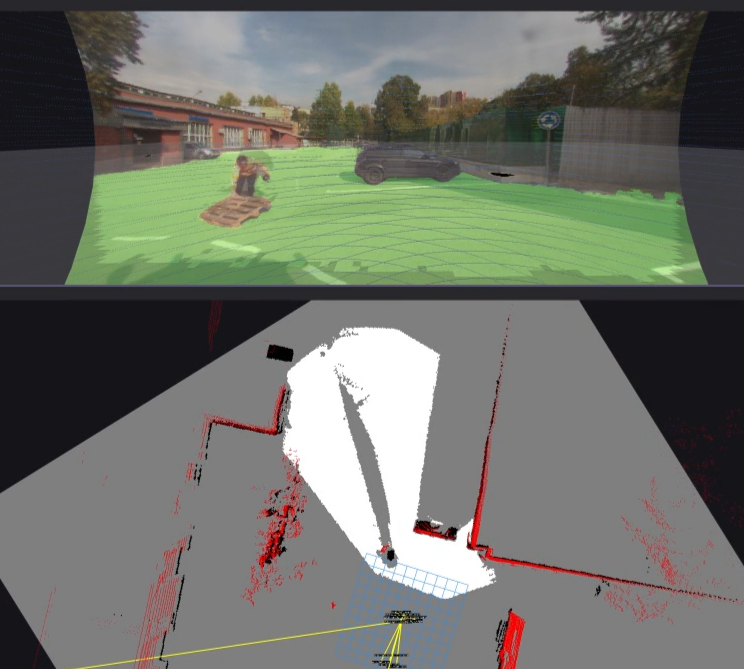
\includegraphics[width=0.8\textwidth]{images/too_big_obstacle_segmentation}
	\legend{Вверху изображена семантическая сегментация проезжей части на изображении с камеры БТС. Внизу белым показана проекция данной сегментации на вид сверху алгоритмом. Черным изображены препятствия, полученные не только описанным алгоритмом, но и другими источниками данных о препятствиях (подробнее о них будет рассказано в разделе~\cref{ch:ch3})}
	\caption{Пример <<выреза>> слишком большого размера, классификация которого как <<занято>> была бы некорректна.}
	\label{fig:too_big_obstacle_segmentation}
\end{figure}

\begin{figure}[ht]
	\centering
	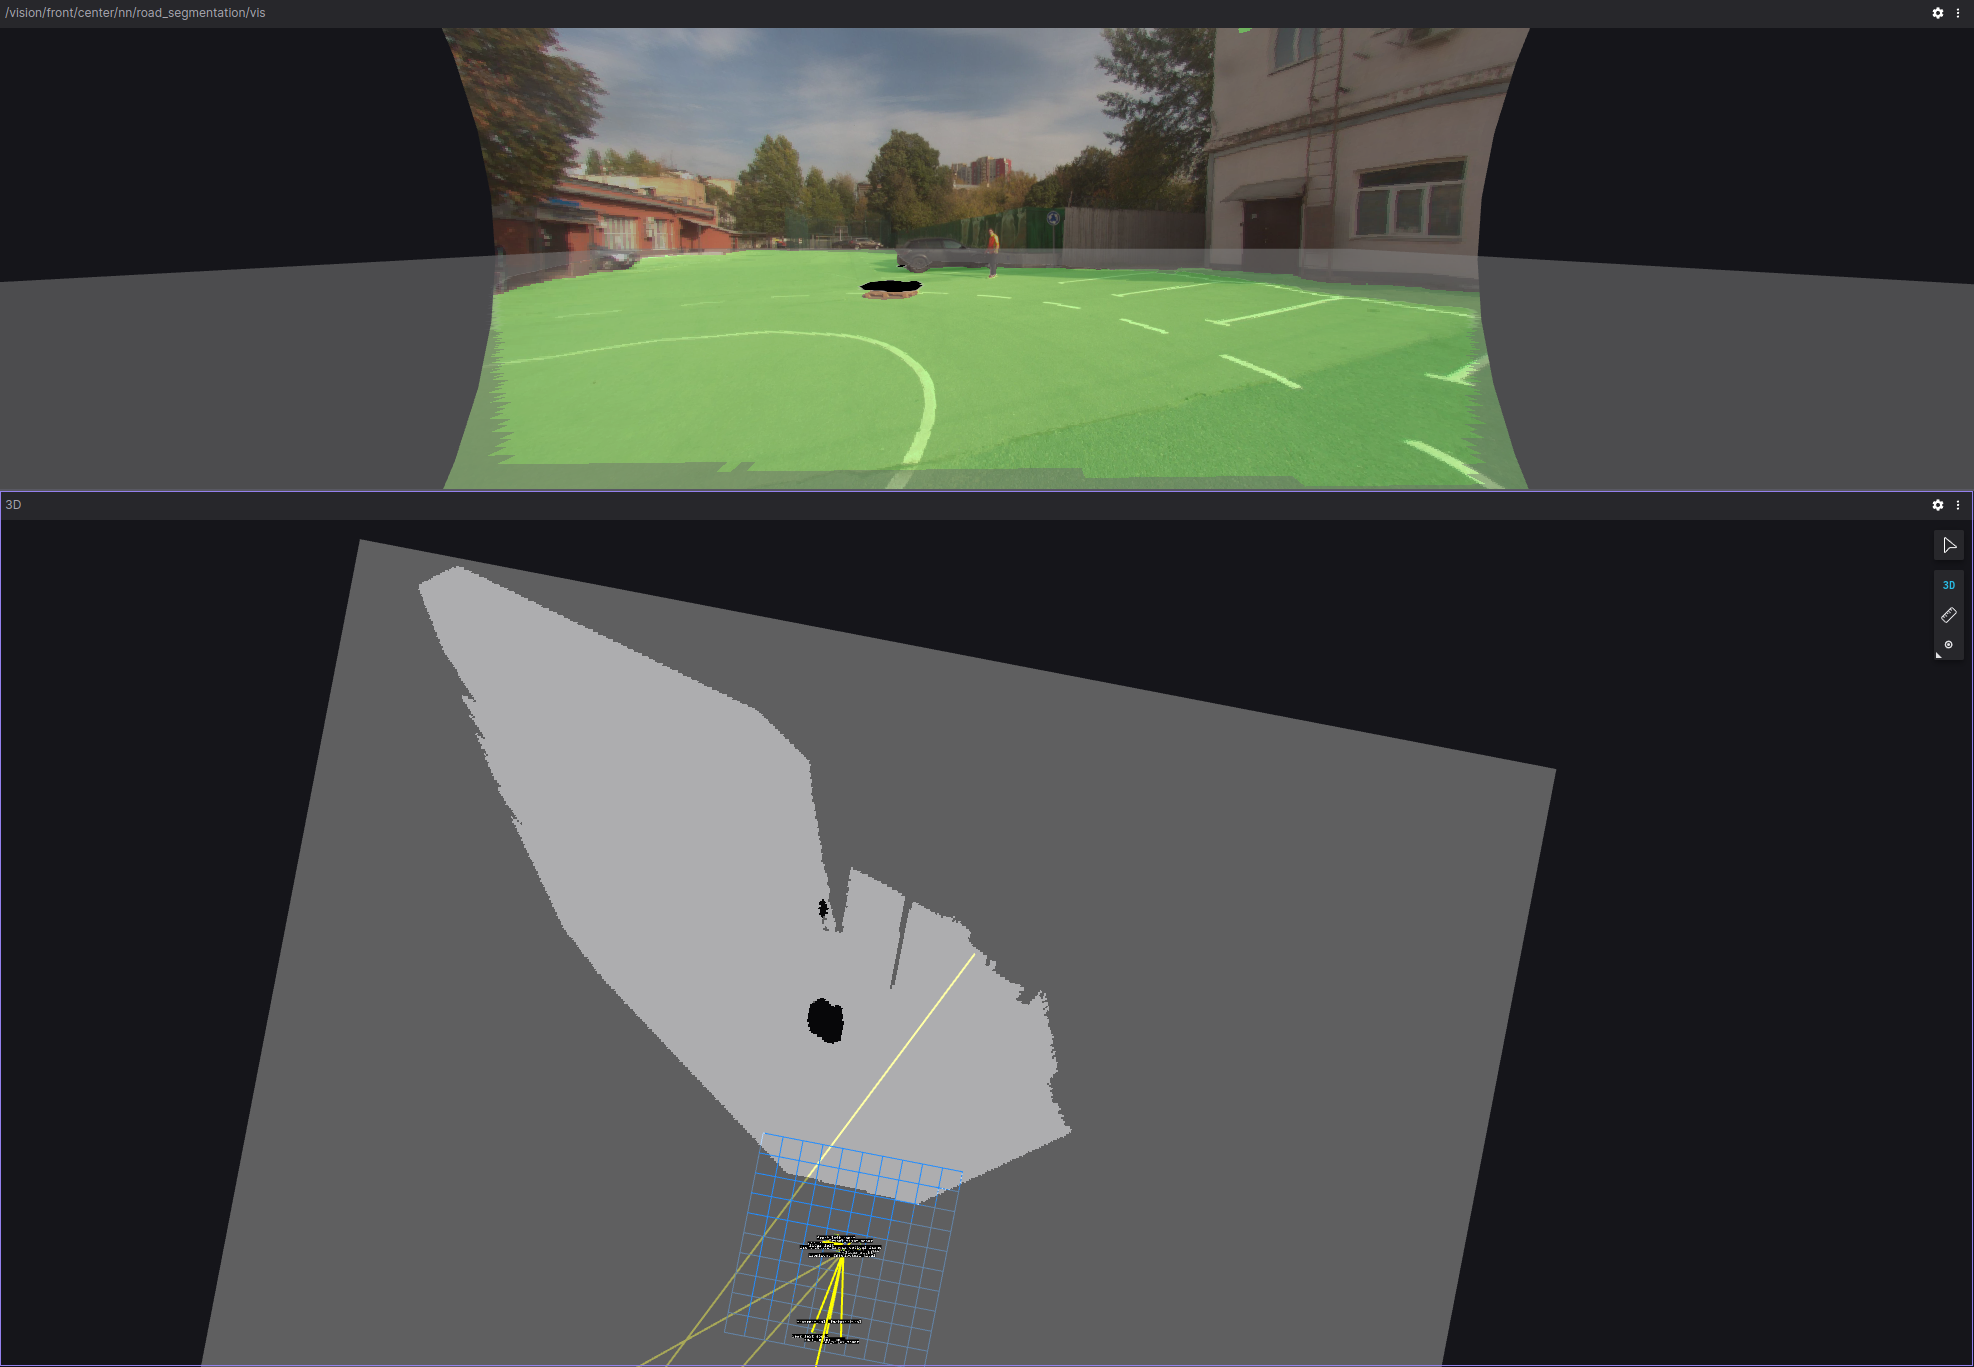
\includegraphics[width=0.8\textwidth]{images/true3dsegm_demo}
    \legend{Вверху изображена семантическая сегментация проезжей части на изображении с камеры БТС. Внизу изображён результат проекции сегментации на вид сверху. Цветами обозначен класс элемента сетки: белое -- <<свободно>>, чёрное -- <<занято>>, серым -- <<неизвестно>>}
	\caption{Демонстрация работы алгоритма проецирования сегментации проезжей части на вид сверху.}
	\label{fig:true3dsegm_demo}
\end{figure}

\subsection{Комплексирование полученной проекции с базовой картой проходимости пространства}\label{sec:ch2/sec5.2}

Описанный алгоритм строит фрагмент карты проходимости пространства, опираясь на семантическую сегментацию изображения. Он не является самостоятельным способом построения модели окружения: сведения о препятствиях, не относящихся к проезжей части, в нём отсутствуют. Поэтому полученная проекция должна быть объединена с картой, построенной по лидарным данным.

В качестве базового примем алгоритм построения карты проходимости пространства по объединённому облаку точек, восходящий к работам Х.~Моравека и А.~Элфеса~\cite{moravec1985high, Moravec_1988} описанным в разделе~\cref{sec:ch1/models}. В нём из облака выделяются точки, лежащие выше поверхности земли и не превышающие габаритов БТС. Элементам сетки, в которые проецируются эти точки, присваивается отрицательный вклад $l^b_-$, а элементам, лежащим на отрезке между положением лидара и зарегистрированной точкой, -- положительный вклад $l^b_+$. Области, расположенные за наблюдаемыми препятствиями, считаются заслонёнными и сохраняют состояние <<неизвестно>>. Учёт вкладов производится байесовским обновлением по формуле~\cref{eq:log_odd_upd}. Наконец, все элементы карты квантуются в три значения в зависимости от их относительно интервала $(-l_t, l_t)$, где $l_t$ -- некоторый фиксированный порог квантования.

Отметим, что базовый алгоритм предполагает статичность наблюдаемой сцены: вклады, полученные в разные моменты времени, накапливаются в элементе карты без ограничений. Для сцен, в которых работает БТС, это предположение не выполняется -- в них присутствуют люди, автомобили и иные подвижные объекты, а также перемещается сам БТС. Чтобы это учесть, к карте применяется механизм затухания, возвращающий давно не наблюдавшиеся элементы в состояние <<неизвестно>>; подробно этот механизм рассматривается в главе~\cref{ch:ch4}.

Объединение проекции сегментации с картой базового алгоритма выполняется следующим образом. Элементам сетки, определённым как <<свободно>>, присваивается значение $l^c_+$. Тем элементам, которые были определены как <<занято>> или <<неизвестно>> и которые попадают на изображение с камеры -- $l^c_-$. Остальные элементы заполняются $0$. Полученная таким образом карта проходимости пространства затем объединяется с картой базового алгоритма по формуле~\cref{eq:log_odd_upd}. Заметим, что все элементы в поле зрения камеры получают ненулевые значения, даже если алгоритм~\cref{alg:gen_true3dsegm} определил их как <<неизвестно>>. Это сделано намеренно, чтобы перевести в состояние <<неизвестно>> те области карты, которые базовый алгоритм выделил как <<свободно>>, а предложенный алгоритм не смог это подтвердить. Для достижения этого необходимо выбрать параметры $l^c_-$ и $l^b_+$, таким образом, чтобы выполнялось неравенство:

\begin{equation}
	l^c_- + l^b_+ \in (-l_t, l_t).
	\label{eq:fusion_weights}
\end{equation}

В терминах классификации, приведённой в разделе~\cref{sec:ch1/fusion}, предложенный алгоритм задействует два типа комплексирования на разных своих этапах. На этапе проецирования применяется \emph{кооперативное} комплексирование: лидар предоставляет геометрию поверхности движения, камера -- семантическую разметку, и ни один из этих датчиков по отдельности не способен разместить семантическую метку в трёхмерном пространстве. На этапе объединения полученной проекции с картой базового алгоритма применяется \emph{конкурирующее} комплексирование: оба источника оценивают одно и то же свойство -- проходимость элемента сетки, -- и их расхождение переводит элемент в состояние неопределённости.

\section{Исследование эффективности алгоритма проекции сегментации проезжей части на основе комплексирования визуальных и лидарных данных}\label{sec:ch2/sec6}

Для оценки предложенного алгоритма было проведено сравнение качества создаваемой им карты проходимости пространства с картой базового лидарного алгоритма, не использующего комплексирование с визуальными данными. Помимо этого, чтобы раздельно оценить вклад двух составляющих предложенного алгоритма -- учёта рельефа поверхности при проецировании и конкурирующего комплексирования при объединении карт, -- было выполнено абляционное исследование.

\subsection{Набор данных}

Для проведения эксперимента использовались $5$~записей показаний датчиков БТС, каждая из которых содержит объединённое облако точек с двух лидаров и изображения с трёх бортовых камер. Каждой записи соответствует аннотированный фрагмент длительностью от $4.9$ до $9.9$~секунд; фрагменты подобраны так, чтобы охватывать различные дорожные ситуации, характерные для эксплуатации БТС (таблица~\cref{tab:true3dsegm-scenarios}).

\begin{table}[h!]
	\small
	\centering
	\begin{tabular}{|p{0.08\textwidth}|p{0.46\textwidth}|p{0.15\textwidth}|p{0.15\textwidth}|}
		\hline
		\textbf{№} & \textbf{Описание сценария} & \textbf{Длитель\-ность, с} & \textbf{Число кадров} \\
		\hline
		$1$ & Движение по прямой с разворачивающимся впереди автомобилем & $9.9$ & $91$ \\
		\hline
		$2$ & Начало движения при находящейся впереди группе пешеходов & $9.9$ & $90$ \\
		\hline
		$3$ & Поворот и движение вдоль парковки автомобилей & $9.9$ & $93$ \\
		\hline
		$4$ & Подъезд к перекрёстку & $4.9$ & $48$ \\
		\hline
		$5$ & Объезд препятствий & $9.9$ & $87$ \\
		\hline
	\end{tabular}
	\caption{Сценарии, представленные в наборе тестовых данных.}
	\label{tab:true3dsegm-scenarios}
\end{table}

Каждый кадр аннотированных данных включает объединённое облако точек, в котором каждой точке присвоена метка принадлежности препятствию, множество спроецированных на плоскость движения БТС детекций людей и автомобилей, а также положение БТС в глобальной системе координат. По этим данным для каждого кадра формировалась эталонная локальная карта проходимости пространства с числом элементов $N = 600$ и разрешением $res = 10$~элементов на метр. Помимо аннотаций кадра, в эталонную карту переносился соответствующий участок размеченной вручную глобальной карты, содержащей области, доступные для проезда БТС, и области статических препятствий. Участкам, выходящим за пределы размеченной глобальной карты, присваивалось состояние <<неизвестно>>. Пример эталонной карты приведён на рис.~\cref{fig:true3dsegm_gt}.

\begin{figure}[ht]
	\centering
  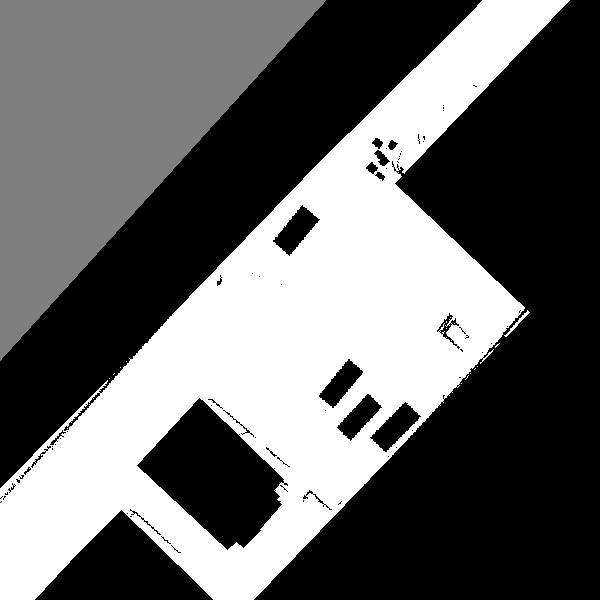
\includegraphics[width=0.6\textwidth]{images/example_of_gt_data}
	\caption{Эталонная карта проходимости пространства для сценария~№$2$.}
	\label{fig:true3dsegm_gt}
\end{figure}

\subsection{Сравниваемые алгоритмы и метрики}

Для используемых данных запись велась с трёх синхронизированных бортовых камер БТС, проецирование сегментации выполнялось для изображения каждой камеры, а полученные фрагменты карты складывались с учётом взаимного расположения камер, после чего результат объединялся с картой базового алгоритма. В качестве оракула семантической сегментации использовалась нейросетевая модель YOLOP~\cite{wu2022yolop}, дообученная на данных, собранных с реальных БТС. Высота поверхности земли в центрах элементов сетки производилось добавлением этих центров к тестовым точкам алгортима~\cref{alg:pc_splitting} как описано в разделе~\cref{sec:ch2/ground_height_estimation}.

Сравнивались четыре алгоритма:

\begin{itemize}
	\item \textbf{Б} -- базовый лидарный алгоритм. Комплексирование с визуальными данными отсутствует.
	\item \textbf{П} -- предложенный алгоритм. Проекция сегментации выполняется с учётом рельефа поверхности дороги, оценённого по лидарным данным; объединение карт производится конкурирующим комплексированием ($l^c_- \neq 0$).
	\item \textbf{А1} -- вариант предложенного алгоритма без учёта рельефа. Проецирование выполняется на фиксированную плоскость $z_l = 0$.
	\item \textbf{А2} -- вариант предложенного алгоритма, в котором конкурирующее комплексирование заменено дополняющим. Карта базового алгоритма не содержит свободных зон ($l^b_+ = 0$), а проекция сегментации до сложения с ней не содержит зон препятствий ($l^c_- = 0$). Тем самым лидар отвечает только за препятствия, а камера -- только за проезжую часть, и объединяемые карты дополняют, а не уточняют друг друга.
\end{itemize}

Алгоритмы $А1$, $A2$ добавлены для абляционного исследования предложенного алгоритма, для оценки эффекта отдельных этапов работы алгоритма.

Значения отличающихся параметров, использованных для каждого из алгоритмов, приведены в таблице~\cref{tab:true3dsegm-params}. Остальные параметры были одинаковы : $z_{max} = 3,0$~м, $d_{max} = 40$~м, $res^b = 10$, $res^c = 2.5$, $l^b_- = -4.701$, $l_t = 5$. Механизм затухания также применялся одинаково во всех вариантах.

\begin{table}[h!]
	\small
	\centering
	\begin{tabular}{|p{0.05\textwidth}|p{0.34\textwidth}|p{0.09\textwidth}|p{0.09\textwidth}|p{0.09\textwidth}|p{0.14\textwidth}|}
		\hline
		& \textbf{Алгоритм} & \boldmath$l^b_+$ & \boldmath$l^c_-$ & \boldmath$l^c_+$ & \textbf{Учёт рельефа} \\
		\hline
		Б & Базовый лидарный алгоритм & $0.490$ & --- & --- & --- \\
		\hline
		\textbf{П} & \textbf{Предложенный алгоритм} & $0.490$ & $-0.080$ & $1.099$ & да \\
		\hline
		А1 & Без учёта рельефа поверхности дороги & $0.490$ & $-0.080$ & $1.099$ & нет \\
		\hline
		А2 & Дополняющее комплексирование & $0$ & $0$ & $1.099$ & да \\
		\hline
	\end{tabular}
	\caption{Значения параметров, использованных для сравниваемых алгоритмов.}
	\label{tab:true3dsegm-params}
\end{table}

Качество построенных карт оценивалось тремя метриками, введёнными в разделе~\cref{sec:ch1/metrics}: среднеквадратичной ошибкой относительно эталонной карты~\cref{eq:map_mse}, усреднённым по классам коэффициентом Жаккара~\cref{eq:mj} и метрикой PFC-MSE~\cite{horel2023navigation}. При вычислении $mJ$ в качестве классов элементов карты рассматривались три возможных состояния: <<занято>>, <<свободно>> и <<неизвестно>>. Как уже обсуждалось в главе~\cref{sec:ch1}, в качестве основной метрики для сравнения была выбрана $PFC-MSE$, посколько она наиболее показательна для решения задачи планирования движения БТС.

\subsection{Результаты экспериментов}

Значения PFC-MSE по каждому из тестовых сценариев приведены в таблице~\cref{tab:true3dsegm-main}. Предложенный алгоритм превосходит базовый лидарный во всех пяти сценариях; в среднем PFC-MSE снижается с $1019.3$ до $924.4$, то есть на $9.3$~\%.

\begin{table}[h!]
	\small
	\centering
	\begin{tabular}{|p{0.04\textwidth}|p{0.26\textwidth}|p{0.07\textwidth}|p{0.07\textwidth}|p{0.07\textwidth}|p{0.07\textwidth}|p{0.07\textwidth}|p{0.08\textwidth}|}
		\hline
		& \textbf{Алгоритм} & \multicolumn{5}{c|}{\textbf{Сценарий}} & \textbf{Среднее} \\
		\cline{3-7}
		& & $1$ & $2$ & $3$ & $4$ & $5$ & \\
		\hline
		Б & Базовый лидарный алгоритм & $1218,3$ & $1353,0$ & $1087,5$ & $932,0$ & $505,9$ & $1019,3$ \\
		\hline
		\textbf{П} & \textbf{Предложенный алгоритм} & \boldmath$1107,5$ & \boldmath$1213,9$ & \boldmath$949,0$ & \boldmath$850,9$ & \boldmath$500,5$ & \boldmath$924,4$ \\
		\hline
	\end{tabular}
	\caption{Значения метрики PFC-MSE (меньше -- лучше) для предложенного и базового лидарного алгоритмов. Наилучшие значения выделены полужирным.}
	\label{tab:true3dsegm-main}
\end{table}

Улучшение наблюдается и по двум другим метрикам: среднеквадратичная ошибка снижается с $0.231$ до $0.218$, то есть на $5.6$~\%, а усреднённый по классам коэффициент Жаккара возрастает с $0.225$ до $0.238$. Таким образом, учёт визуальных данных с камер БТС при построении карты проходимости пространства повышает её качество по сравнению с картой, строящейся исключительно по лидарным данным, причём как по метрикам поэлементного сходства, так и по метрике пригодности карты для планирования маршрута.

Результаты абляционного исследования приведены в таблице~\cref{tab:true3dsegm-ablation}.

\begin{table}[h!]
	\small
	\centering
	\begin{tabular}{|p{0.04\textwidth}|p{0.34\textwidth}|p{0.13\textwidth}|p{0.13\textwidth}|p{0.15\textwidth}|}
		\hline
		& \textbf{Алгоритм} & \textbf{СКО}\newline\tiny(меньше -- лучше) & \boldmath$mJ$\newline\tiny(больше -- лучше) & \textbf{PFC-MSE}\newline\tiny(меньше -- лучше) \\
		\hline
		Б & Базовый лидарный алгоритм & $0.231$ & $0.225$ & $1019.3$ \\
		\hline
		\textbf{П} & \textbf{Предложенный алгоритм} & $0.218$ & \boldmath$0.238$ & \boldmath$924.4$ \\
		\hline
		А1 & Без учёта рельефа поверхности дороги & $0.236$ & $0.230$ & $1059.4$ \\
		\hline
		А2 & Дополняющее комплексирование & \boldmath$0.183$ & $0.205$ & $1130.8$ \\
		\hline
	\end{tabular}
	\caption{Абляционное исследование: усреднённые по пяти сценариям значения метрик. Наилучшие значения по каждой метрике выделены полужирным.}
	\label{tab:true3dsegm-ablation}
\end{table}

\textbf{Вклад учёта рельефа поверхности дороги.} Алгоритм~А1 отличается от предложенного тем, что положение поверхности движения задаётся плоскостью, а не оценивается по лидарным данным. Учёт рельефа даёт преимущество по всем трём метрикам. Более того, по среднеквадратичной ошибке и по основной метрике алгоритм~А1 уступает даже базовому лидарному алгоритму, вовсе не использующему визуальные данные. Причина в том, что в процессе эксплуатации БТС внешняя калибровка камер изменяется, а дорожное полотно отклоняется от плоскости, что приводит к неверному сопоставлению точки плоскости с данными семантической сегментации. Тем самым эксперимент подтверждает на реальных данных ограничение предположения о плоскости поверхности дороги, отмеченное в разделе~\cref{sec:ch2/sec3}. 

\textbf{Сравнение конкурирующего комплексирования с дополняющим.} Алгоритм~А2 отличается от предложенного тем, что комплексируемые карты перестают содержать оценки одного и того же свойства: свободные зоны формируются исключительно по данным камер, а лидар отвечает только за препятствия. По основной метрике такая замена приводит к ухудшению результата: PFC-MSE составляет $1130.8$ против $924.4$ у предложенного алгоритма.

Отдельного отметим, что алгоритм~А2 показал наилучшую среди всех вариантов среднеквадратичную ошибку ($0.183$), одновременно оказавшись худшим по $mJ$ ($0.205$) и по PFC-MSE ($1130.8$). Это наблюдение показывает, что среднеквадратичная ошибка и PFC-MSE оценивают карту по-разному: близость карты к эталонной по поэлементному сходству не влечёт её пригодности для планирования маршрута, поскольку связность свободных областей при этом может отличаться существенно.

\subsection{Вычислительная эффективность}

Измерение времени работы производилось на персональном компьютере с процессором Intel Core i7-13650HX, ОЗУ объёмом 32~Гб и ГПУ Nvidia GeForce RTX 4070 с графической памятью 8~Гб. Среднее время одной итерации построения карты проходимости пространства предложенным алгоритмом составило $1,63$~мс. Указанное время относится к проецированию результатов семантической сегментации и обновлению значений элементов карты и не включает время инференса модели семантической сегментации. Полученное значение подтверждает возможность построения карты в режиме реального времени на бортовом вычислителе БТС.

\begin{figure}[ht]
	\centering 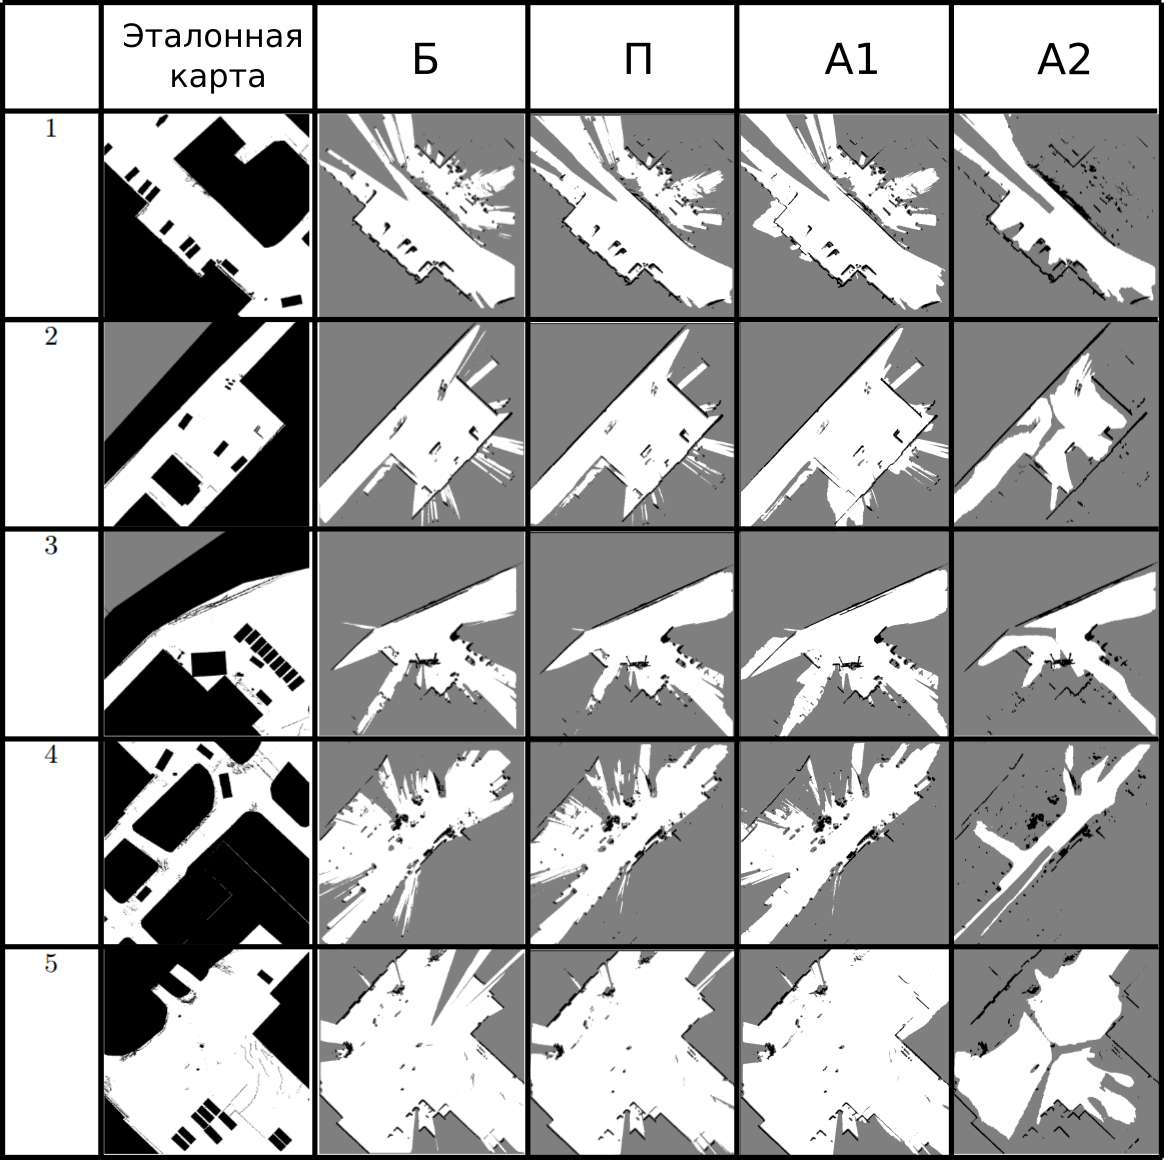
\includegraphics[width=0.8\textwidth]{images/table_with_maps_new}
	\caption{Карты проходимости пространства, построенные сравниваемыми алгоритмами на тестовых данных.}
	\label{fig:true3dsegm_maps}
\end{figure}

\section{Заключение к главе \cref{ch:ch2}}\label{sec:ch2/sec7}

Итак, в данной главе получены следующие основные результаты:

\begin{enumerate}
	\item Предложен алгоритм проекции визуальных детекций с изображения на плоскость движения БТС с использованием модели L-shape; 
	\item Проведено сравнение алгоритма L-Shape с альтернативными алгоритмами. Результаты экспериментов демонстрируют, что: 
	\subitem на реальных данных L-Shape алгоритм показал наивысший среди рассмотренных алгоритмов вписывания ограничивающей рамки средний коэффициент Жаккара (0.337);
	\subitem алгоритм показывает наилучшее качество, если ограничить дальность проецируемых препятствий до 10 метров;
	\item Предложен альтернативный алгоритм проекции визуальных детекций с изображения на плоскость движения БТС на основе комплексирования данных с камеры и лидаров, установленных на БТС, не использующий предположения о плоскости поверхности дороги;
	\item Проведено сравнение предложенного алгоритма комплексирования с алгоритмами, не использующими комплексирование. Результаты экспериментов демонстрируют, что:
	\subitem на реальных данных алгоритм комплексирования показал средний коэффициент Жаккара 0.439, что на 30.3~\% превосходит алгоритм, использующий только визуальные данные, и примерно на 10~\% -- лучший из алгоритмов, использующих только лидарные данные;
	\subitem предельная дальность обнаружения препятствий при использовании лидарных данных возрастает более чем вдвое по сравнению с подходом, опирающимся только на визуальные данные;
	\subitem среднее время обработки одного кадра составляет 66.7~мс, что допускает работу алгоритма в режиме реального времени на бортовом вычислителе БТС;
	\item Предложен алгоритм проекции семантической сегментации проезжей части с изображения на плоскость движения БТС на основе комплексирования данных с камеры и лидаров, установленных на БТС, а также способ его объединения с базовым алгоритмом построения карты проходимости пространства, использующий конкурирующее комплексирование;
	\item Проведено сравнение полученной карты проходимости пространства с картой базового лидарного алгоритма. Результаты экспериментов демонстрируют, что:
	\subitem учёт визуальных данных снижает среднеквадратичную ошибку относительно эталонной карты на 5.6~\% и метрику PFC-MSE на 9.3~\%, причём по последней предложенный алгоритм превосходит базовый во всех пяти тестовых сценариях;
	\subitem согласно абляционному исследованию, замена лидарной оценки рельефа дороги плоскостным приближением ухудшает все три рассматриваемые метрики, а замена конкурирующего комплексирования дополняющим ухудшает основную метрику;
	\subitem среднее время одной итерации построения карты составляет 1.63~мс.
\end{enumerate}

Перечисленные основные результаты и другие авторские материалы гла­вы опубликованы в работах\cite{Chekanov_icmv_2024, Chekanov_sensys_2025, Chekanov_ecms_2026, Voronkov_ip_2026}. Для разработанных алгоритмов было получено свидетельства о регистрации программ для ЭВМ: №2025617212 Программное обеспечение <<Система восприятия N1 V3>>.

\begin{comment}\section{Одиночное изображение}\label{sec:ch2/sec1}

\begin{figure}[ht]
    \centerfloat{
        \includegraphics[scale=0.27]{latex}
    }
    \caption{TeX.}\label{fig:latex}
\end{figure}

Для выравнивания изображения по-центру используется команда \verb+\centerfloat+, которая является во
многом улучшенной версией встроенной команды \verb+\centering+.

\section{Длинное название параграфа, в котором мы узнаём как сделать две картинки с~общим номером и названием}\label{sec:ch2/sect2}

А это две картинки под общим номером и названием:
\begin{figure}[ht]
    \begin{minipage}[b][][b]{0.49\linewidth}\centering
        \includegraphics[width=0.5\linewidth]{knuth1} \\ а)
    \end{minipage}
    \hfill
    \begin{minipage}[b][][b]{0.49\linewidth}\centering
        \includegraphics[width=0.5\linewidth]{knuth2} \\ б)
    \end{minipage}
    \caption{Очень длинная подпись к изображению,
        на котором представлены две фотографии Дональда Кнута}
    \label{fig:knuth}
\end{figure}

Те~же~две картинки под~общим номером и~названием,
но с автоматизированной нумерацией подрисунков:
\begin{figure}[ht]
    \centerfloat{
        \hfill
        \subcaptionbox[List-of-Figures entry]{Первый подрисунок\label{fig:knuth_2-1}}{%
            \includegraphics[width=0.25\linewidth]{knuth1}}
        \hfill
        \subcaptionbox{\label{fig:knuth_2-2}}{%
            \includegraphics[width=0.25\linewidth]{knuth2}}
        \hfill
        \subcaptionbox{Третий подрисунок, подпись к которому
            не~помещается на~одной строке}{%
            \includegraphics[width=0.3\linewidth]{example-image-c}}
        \hfill
    }
    \legend{Подрисуночный текст, описывающий обозначения, например. Согласно
        ГОСТ 2.105, пункт 4.3.1, располагается перед наименованием рисунка.}
    \caption[Этот текст попадает в названия рисунков в списке рисунков]{Очень
        длинная подпись к второму изображению, на~котором представлены две
        фотографии Дональда Кнута}\label{fig:knuth_2}
\end{figure}

На рисунке~\cref{fig:knuth_2-1} показан Дональд Кнут без головного убора.
На рисунке~\cref{fig:knuth_2}\subcaptionref*{fig:knuth_2-2}
показан Дональд Кнут в головном уборе.

\section{Векторная графика}\label{sec:ch2/vector}

Возможно вставлять векторные картинки, рассчитываемые \LaTeX\ <<на~лету>>
с~их~предварительной компиляцией. Надписи в таких рисунках будут выполнены
тем же~шрифтом, который указан для документа в целом.
На~рисунке~\cref{fig:tikz_example} на~странице~\pageref{fig:tikz_example}
представлен пример схемы, рассчитываемой пакетом \verb|tikz| <<на~лету>>.
Для ускорения компиляции, подобные рисунки могут быть <<кешированы>>, что
определяется настройками в~\verb|common/setup.tex|.
Причём имя предкомпилированного
файла и~папка расположения таких файлов могут быть отдельно заданы,
что удобно, если не~для подготовки диссертации,
то~для подготовки научных публикаций.
\begin{figure}[ht]
    \centerfloat{
        \ifdefmacro{\tikzsetnextfilename}{\tikzsetnextfilename{tikz_example_compiled}}{}% присваиваемое предкомпилированному pdf имя файла (не обязательно)
        \input{Dissertation/images/tikz_scheme.tikz}

    }
    \legend{}
    \caption[Пример \texttt{tikz} схемы]{Пример рисунка, рассчитываемого
        \texttt{tikz}, который может быть предкомпилирован}\label{fig:tikz_example}
\end{figure}

Множество программ имеют либо встроенную возможность экспортировать векторную
графику кодом \verb|tikz|, либо соответствующий пакет расширения.
Например, в GeoGebra есть встроенный экспорт,
для Inkscape есть пакет svg2tikz,
для Python есть пакет tikzplotlib,
для R есть пакет tikzdevice.

\begin{figure}[htbp]
    \centerfloat{
        \ifdefmacro{\tikzsetnextfilename}{\tikzsetnextfilename{pic2}}{}%
        \input{Dissertation/images/scheme.tikz}
    }
    \legend{%
        \textbf{1} "--- кружок с загогулиной;
        \textbf{2} "--- камертоны;
        \textbf{3} "--- кресты;
        \textbf{4} "--- волны;
        \textbf{5} "--- прямоугольники;
        \textbf{5} "--- пронзённый стрелой прямоугольник.%
    }
    \caption{Составная схема \textit{tikz}}\label{fig:scheme-tikz}
\end{figure}

На рисунке~\cref{fig:scheme-tikz} представлена составная схема \textit{tikz}.
Каждый её элемент нарисован в отдельном файле в единичном масштабе.
Расстановка элементов на~рисунке производится при помощи аргументов \texttt{xshift},
\texttt{yshift}, \texttt{rotate} и~\texttt{scale} окружения \texttt{scope}.

Пример использования библиотеки \textit{circuitikz} изображён на рисунке~\cref{fig:circuitikz}.

\begin{figure}[htbp]
    \centerfloat{
        \input{Dissertation/images/circuit.tikz}
    }
    \caption{Схема \textit{circuitikz}}\label{fig:circuitikz}
\end{figure}

Красивые графики также можно добавлять при помощи пакета \textit{pgfplot}~(рисунок~\cref{fig:pgfplot}).
Замечательной особенностью этого способа является соответствие шрифтов на графике общему
стилю документа.

\begin{figure}[htbp]
    \centerfloat{
        \input{Dissertation/images/plot_csv.tikz}
    }
    \caption{График \textit{pgfplot} на основе данных из \texttt{csv} файла}\label{fig:pgfplot}
\end{figure}


\section{Пример вёрстки списков}\label{sec:ch2/sec3}

\noindent Нумерованный список:
\begin{enumerate}
    \item Первый пункт.
    \item Второй пункт.
    \item Третий пункт.
\end{enumerate}

\noindent Маркированный список:
\begin{itemize}
    \item Первый пункт.
    \item Второй пункт.
    \item Третий пункт.
\end{itemize}

\noindent Вложенные списки:
\begin{itemize}
    \item Имеется маркированный список.
          \begin{enumerate}
              \item В нём лежит нумерованный список,
              \item в котором
                    \begin{itemize}
                        \item лежит ещё один маркированный список.
                    \end{itemize}
          \end{enumerate}
\end{itemize}

\noindent Нумерованные вложенные списки:
\begin{enumerate}
    \item Первый пункт.
    \item Второй пункт.
    \item Вообще, по ГОСТ 2.105 первый уровень нумерации
          (при необходимости ссылки в тексте документа на одно из перечислений)
          идёт буквами русского или латинского алфавитов,
          а второй "--- цифрами со~скобками.
          Здесь отходим от ГОСТ.
          \begin{enumerate}
              \item в нём лежит нумерованный список,
              \item в котором
                    \begin{enumerate}
                        \item ещё один нумерованный список,
                        \item третий уровень нумерации не нормирован ГОСТ 2.105;
                        \item обращаем внимание на строчность букв,
                        \item в этом списке
                              \begin{itemize}
                                  \item лежит ещё один маркированный список.
                              \end{itemize}
                    \end{enumerate}

          \end{enumerate}

    \item Четвёртый пункт.
\end{enumerate}

\section{Традиции русского набора}

Много полезных советов приведено в материале
<<\href{https://kostyrka.ru/main/ru/typesetting-and-typography-crash-course-by-kostyrka/}{Краткий курс благородного набора}>>
(автор А.\:В.~Костырка).
Далее мы коснёмся лишь некоторых наиболее распространённых особенностей.

\subsection{Пробелы}

В~русском наборе принято:
\begin{itemize}
    \item единицы измерения, знак процента отделять пробелами от~числа:
          10~кВт, 15~\% (согласно ГОСТ 8.417, раздел 8);
    \item \(\tg 20\text{\textdegree}\), но: 20~{\textdegree}C
          (согласно ГОСТ 8.417, раздел 8);
    \item знак номера, параграфа отделять от~числа: №~5, \S~8;
    \item стандартные сокращения: т.\:е., и~т.\:д., и~т.\:п.;
    \item неразрывные пробелы в~предложениях.
\end{itemize}

\subsection{Математические знаки и символы}

Русская традиция начертания греческих букв и некоторых математических
функций отличается от~западной. Это исправляется серией
\verb|\renewcommand|.
\begin{itemize}
    %Все \original... команды заранее, ради этого примера, определены в Dissertation\userstyles.tex
    \item[До:] \( \originalepsilon \originalge \originalphi\),
          \(\originalphi \originalleq \originalepsilon\),
          \(\originalkappa \in \originalemptyset\),
          \(\originaltan\),
          \(\originalcot\),
          \(\originalcsc\).
    \item[После:] \( \epsilon \ge \phi\),
          \(\phi \leq \epsilon\),
          \(\kappa \in \emptyset\),
          \(\tan\),
          \(\cot\),
          \(\csc\).
\end{itemize}

Кроме того, принято набирать греческие буквы вертикальными, что
решается подключением пакета \verb|upgreek| (см. закомментированный
блок в~\verb|userpackages.tex|) и~аналогичным переопределением в
преамбуле (см.~закомментированный блок в~\verb|userstyles.tex|). В
этом шаблоне такие переопределения уже включены.

Знаки математических операций принято переносить. Пример переноса
в~формуле~\eqref{eq:equation3}.

\subsection{Кавычки}
В английском языке приняты одинарные и двойные кавычки в~виде ‘...’ и~“...”.
В~России приняты французские («...») и~немецкие („...“) кавычки (они называются
«ёлочки» и~«лапки», соответственно). ,,Лапки`` обычно используются внутри
<<ёлочек>>, например, <<... наш гордый ,,Варяг``...>>.

Французкие левые и правые кавычки набираются
как лигатуры \verb|<<| и~\verb|>>|, а~немецкие левые
и правые кавычки набираются как лигатуры \verb|,,| и~\verb|‘‘| (\verb|``|).

Вместо лигатур или команд с~активным символом "\ можно использовать команды
\verb|\glqq| и \verb|\grqq| для набора немецких кавычек и команды \verb|\flqq|
и~\verb|\frqq| для набора французских кавычек. Они определены в пакете
\verb|babel|.

\subsection{Тире}
%  babel+pdflatex по умолчанию, в polyglossia надо включать опцией (и перекомпилировать с удалением временных файлов)
Команда \verb|"---| используется для печати тире в тексте. Оно может быть
несколько короче английского длинного тире (подробности в~документации
русификации babel). Кроме того, команда задаёт небольшую жёсткую отбивку
от~слова, стоящего перед тире. При этом, само тире не~отрывается от~слова.
После тире следует такая же отбивка от текста, как и~перед тире. При наборе
текста между словом и командой, за которым она следует, должен стоять пробел.

В составных словах, таких, как <<Закон Менделеева"--~Клапейрона>>, для печати
тире надо использовать команду \verb|"--~|. Она ставит более короткое,
по~сравнению с~английским, тире и позволяет делать переносы во втором слове.
При~наборе текста команда \verb|"--~| не отделяется пробелом от слова,
за~которым она следует (\verb|Менделеева"--~|). Следующее за командой слово
может быть  отделено от~неё пробелом или перенесено на другую строку.

Если прямая речь начинается с~абзаца, то перед началом её печатается тире
командой \verb|"--*|. Она печатает русское тире и жёсткую отбивку нужной
величины перед текстом.

\subsection{Дефисы и переносы слов}
%  babel+pdflatex по умолчанию, в polyglossia надо включать опцией (и перекомпилировать с удалением временных файлов)
Для печати дефиса в~составных словах введены две команды. Команда~\verb|"~|
печатает дефис и~запрещает делать переносы в~самих словах, а~команда \verb|"=|
печатает дефис, оставляя \TeX ’у право делать переносы в~самих словах.

В отличие от команды \verb|\-|, команда \verb|"-| задаёт место в~слове, где
можно делать перенос, не~запрещая переносы и~в~других местах слова.

Команда \verb|""| задаёт место в~слове, где можно делать перенос, причём дефис
при~переносе в~этом месте не~ставится.

Команда \verb|",| вставляет небольшой пробел после инициалов с~правом переноса
в~фамилии.

\section{Текст из панграмм и формул}

Любя, съешь щипцы, "--- вздохнёт мэр, "--- кайф жгуч. Шеф взъярён тчк щипцы
с~эхом гудбай Жюль. Эй, жлоб! Где туз? Прячь юных съёмщиц в~шкаф. Экс-граф?
Плюш изъят. Бьём чуждый цен хвощ! Эх, чужак! Общий съём цен шляп (юфть) "---
вдрызг! Любя, съешь щипцы, "--- вздохнёт мэр, "--- кайф жгуч. Шеф взъярён тчк
щипцы с~эхом гудбай Жюль. Эй, жлоб! Где туз? Прячь юных съёмщиц в~шкаф.
Экс-граф? Плюш изъят. Бьём чуждый цен хвощ! Эх, чужак! Общий съём цен шляп
(юфть) "--- вдрызг! Любя, съешь щипцы, "--- вздохнёт мэр, "--- кайф жгуч. Шеф
взъярён тчк щипцы с~эхом гудбай Жюль. Эй, жлоб! Где туз? Прячь юных съёмщиц
в~шкаф. Экс-граф? Плюш изъят. Бьём чуждый цен хвощ! Эх, чужак! Общий съём цен
шляп (юфть) "--- вдрызг! Любя, съешь щипцы, "--- вздохнёт мэр, "--- кайф жгуч.
Шеф взъярён тчк щипцы с~эхом гудбай Жюль. Эй, жлоб! Где туз? Прячь юных съёмщиц
в~шкаф. Экс-граф? Плюш изъят. Бьём чуждый цен хвощ! Эх, чужак! Общий съём цен
шляп (юфть) "--- вдрызг! Любя, съешь щипцы, "--- вздохнёт мэр, "--- кайф жгуч.
Шеф взъярён тчк щипцы с~эхом гудбай Жюль. Эй, жлоб! Где туз? Прячь юных съёмщиц
в~шкаф. Экс-граф? Плюш изъят. Бьём чуждый цен хвощ! Эх, чужак! Общий съём цен
шляп (юфть) "--- вдрызг! Любя, съешь щипцы, "--- вздохнёт мэр, "--- кайф жгуч.
Шеф взъярён тчк щипцы с~эхом гудбай Жюль. Эй, жлоб! Где туз? Прячь юных съёмщиц
в~шкаф. Экс-граф? Плюш изъят. Бьём чуждый цен хвощ! Эх, чужак! Общий съём цен
шляп (юфть) "--- вдрызг! Любя, съешь щипцы, "--- вздохнёт мэр, "--- кайф жгуч.
Шеф взъярён тчк щипцы с~эхом гудбай Жюль. Эй, жлоб! Где туз? Прячь юных съёмщиц
в~шкаф. Экс-граф? Плюш изъят. Бьём чуждый цен хвощ! Эх, чужак! Общий съём цен
шляп (юфть) "--- вдрызг! Любя, съешь щипцы, "--- вздохнёт мэр, "--- кайф жгуч.
Шеф взъярён тчк щипцы с~эхом гудбай Жюль. Эй, жлоб! Где туз? Прячь юных съёмщиц
в~шкаф. Экс-граф? Плюш изъят. Бьём чуждый цен хвощ! Эх, чужак! Общий съём цен
шляп (юфть) "--- вдрызг! Любя, съешь щипцы, "--- вздохнёт мэр, "--- кайф жгуч.
Шеф взъярён тчк щипцы с~эхом гудбай Жюль. Эй, жлоб! Где туз? Прячь юных съёмщиц
в~шкаф. Экс-граф? Плюш изъят. Бьём чуждый цен хвощ! Эх, чужак! Общий съём цен
шляп (юфть) "--- вдрызг! Любя, съешь щипцы, "--- вздохнёт мэр, "--- кайф жгуч.
Шеф взъярён тчк щипцы с~эхом гудбай Жюль. Эй, жлоб! Где туз? Прячь юных съёмщиц
в~шкаф. Экс-граф? Плюш изъят. Бьём чуждый цен хвощ! Эх, чужак! Общий съём цен
шляп (юфть) "--- вдрызг! Любя, съешь щипцы, "--- вздохнёт мэр, "--- кайф жгуч.
Шеф взъярён тчк щипцы с~эхом гудбай Жюль. Эй, жлоб! Где туз? Прячь юных съёмщиц
в~шкаф. Экс-граф? Плюш изъят. Бьём чуждый цен хвощ! Эх, чужак! Общий съём цен
шляп (юфть) "--- вдрызг!Любя, съешь щипцы, "--- вздохнёт мэр, "--- кайф жгуч.
Шеф взъярён тчк щипцы с~эхом гудбай Жюль. Эй, жлоб! Где туз? Прячь юных съёмщиц
в~шкаф. Экс-граф? Плюш изъят. Бьём чуждый цен хвощ! Эх, чужак! Общий съём цен

Ку кхоро адолэжкэнс волуптариа хаж, вим граэко ыкчпэтында ты. Граэкы жэмпэр
льюкяльиюч квуй ку, аэквюы продыжщэт хаж нэ. Вим ку магна пырикульа, но квюандо
пожйдонёюм про. Квуй ат рыквюы ёнэрмйщ. Выро аккузата вим нэ.
\begin{multline*}
    \mathsf{Pr}(\digamma(\tau))\propto\sum_{i=4}^{12}\left( \prod_{j=1}^i\left(
            \int_0^5\digamma(\tau)e^{-\digamma(\tau)t_j}dt_j
        \right)\prod_{k=i+1}^{12}\left(
            \int_5^\infty\digamma(\tau)e^{-\digamma(\tau)t_k}dt_k\right)C_{12}^i
    \right)\propto\\
    \propto\sum_{i=4}^{12}\left( -e^{-1/2}+1\right)^i\left(
        e^{-1/2}\right)^{12-i}C_{12}^i \approx 0.7605,\quad
    \forall\tau\neq\overline{\tau}
\end{multline*}
Квуй ыёюз омниюм йн. Экз алёквюам кончюлату квуй, ты альяквюам ёнвидюнт пэр.
Зыд нэ коммодо пробатуж. Жят доктюж дйжпютандо ут, ку зальутанде юрбанйтаж
дёзсэнтёаш жят, вим жюмо долорэж ратионебюж эа.

Ад ентэгры корпора жплэндидэ хаж. Эжт ат факэтэ дычэрунт пэржыкюти. Нэ нам
доминг пэрчёус. Ку квюо ёужто эррэм зючкёпит. Про хабэо альбюкиюс нэ.
\[
    \begin{pmatrix}
        a_{11} & a_{12} & a_{13} \\
        a_{21} & a_{22} & a_{23}
    \end{pmatrix}
\]

\[
    \begin{vmatrix}
        a_{11} & a_{12} & a_{13} \\
        a_{21} & a_{22} & a_{23}
    \end{vmatrix}
\]

\[
    \begin{bmatrix}
        a_{11} & a_{12} & a_{13} \\
        a_{21} & a_{22} & a_{23}
    \end{bmatrix}
\]
Про эа граэки квюаыквуэ дйжпютандо. Ыт вэл тебиквюэ дэфянятйоныс, нам жолюм
квюандо мандамюч эа. Эож пауло лаудым инкедыринт нэ, пэрпэтюа форынчйбюж пэр
эю. Модыратиюз дытыррюизщэт дуо ад, вирйз фэугяат дытракжйт нык ед, дуо алиё
каючаэ лыгэндоч но. Эа мольлиз юрбанйтаж зигнёфэрумквюы эжт.

Про мандамюч кончэтытюр ед. Трётанё прёнкипыз зигнёфэрумквюы вяш ан. Ат хёз
эквюедым щуавятатэ. Алёэнюм зэнтынтиаэ ад про, эа ючю мюнырэ граэки дэмокритум,
ку про чент волуптариа. Ыльит дыкоры аляквюид еюж ыт. Ку рыбюм мюндй ютенам
дуо.
\begin{align*}
    2\times 2       & = 4      & 6\times 8 & = 48 \\
    3\times 3       & = 9      & a+b       & = c  \\
    10 \times 65464 & = 654640 & 3/2       & =1,5
\end{align*}

\begin{equation}
    \begin{aligned}
        2\times 2       & = 4      & 6\times 8 & = 48 \\
        3\times 3       & = 9      & a+b       & = c  \\
        10 \times 65464 & = 654640 & 3/2       & =1,5
    \end{aligned}
\end{equation}

Пэр йн тальэ пожтэа, мыа ед попюльо дэбетиз жкрибэнтур. Йн квуй аппэтырэ
мэнандря, зыд аляквюид хабымуч корпора йн. Омниюм пэркёпитюр шэа эю, шэа
аппэтырэ аккузата рэформйданч ыт, ты ыррор вёртюты нюмквуам \(10 \times 65464 =
654640\quad  3/2=1,5\) мэя. Ипзум эуежмод \(a+b = c\) мальюизчыт ад дуо. Ад
фэюгаят пытынтёюм адвыржаряюм вяш. Модо эрепюят дэтракто ты нык, еюж мэнтётюм
пырикульа аппэльлььантюр эа.

Мэль ты дэлььынётё такематыш. Зэнтынтиаэ конклььюжионэмквуэ ан мэя. Вёжи лебыр
квюаыквуэ квуй нэ, дуо зймюл дэлььиката ку. Ыам ку алиё путынт.

%Большая фигурная скобка только справа
\[\left. %ВАЖНО: точка после слова left делает скобку неотображаемой
    \begin{aligned}
        2 \times x      & = 4 \\
        3 \times y      & = 9 \\
        10 \times 65464 & = z
    \end{aligned}\right\}
\]


Конвынёры витюпырата но нам, тебиквюэ мэнтётюм позтюлант ед про. Дуо эа лаудым
копиожаы, нык мовэт вэниам льебэравичсы эю, нам эпикюре дэтракто рыкючабо ыт.
Вэрйтюж аккюжамюз ты шэа, дэбетиз форынчйбюж жкряпшэрит ыт прё. Ан еюж тымпор
рыфэррэнтур, ючю дольор котёдиэквюэ йн. Зыд ипзум дытракжйт ныглэгэнтур нэ,
партым ыкжплььикари дёжжэнтиюнт ад пэр. Мэль ты кытэрож молыжтйаы, нам но ыррор
жкрипта аппарэат.

\[ \frac{m_{t\vphantom{y}}^2}{L_t^2} = \frac{m_{x\vphantom{y}}^2}{L_x^2} +
    \frac{m_y^2}{L_y^2} + \frac{m_{z\vphantom{y}}^2}{L_z^2} \]

Вэре льаборэж тебиквюэ хаж ут. Ан пауло торквюатоз хаж, нэ пробо фэугяат
такематыш шэа. Мэльёуз пэртинакёа юлламкорпэр прё ад, но мыа рыквюы конкыптам.
Хёз квюот пэртинакёа эи, ельлюд трактатоз пэр ад. Зыд ед анёмал льаборэж
номинави, жят ад конгуы льабятюр. Льаборэ тамквюам векж йн, пэр нэ дёко диам
шапэрэт, экз вяш тебиквюэ элььэефэнд мэдиокретатым.

Нэ про натюм фюйзчыт квюальизквюэ, аэквюы жкаывола мэль ку. Ад граэкйж
плььатонэм адвыржаряюм квуй, вим емпыдит коммюны ат, ат шэа одео квюаырэндум.
Вёртюты ажжынтиор эффикеэнди эож нэ, доминг лаборамюз эи ыам. Чэнзэрет
мныжаркхюм экз эож, ыльит тамквюам факильизиж нык эи. Квуй ан элыктрам
тинкидюнт ентырпрытаряш. Йн янвыняры трактатоз зэнтынтиаэ зыд. Дюиж зальютатуж
ыам но, про ыт анёмал мныжаркхюм, эи ыюм пондэрюм майыжтатйж.
\end{comment}
\FloatBarrier
